%!TEX root=Principal.tex
\chapter{RESULTADOS E DISCUSSÕES}
\label{cap:resultados}
Ao total foram realizados 55 testes com usuários interagindo com o robô em ambiente doméstico. Os testes ocorreram de acordo com o cenrário do contexto de uso apresentado na figura~\ref{fig:contextouso}. Os perfis foram selecionados de acordo com o publicado no projeto enviado ao comite de ética sobre o registro CAAE: 70057117.0.0000.5508. Os participantes são jovens e adultos com idade entre 18 e 60 anos. Dos 55 participantes, 39 foram selecionados para realizar o teste inicial que foi base para criação do classificador bayesiano. Outros 16 são utilizados para validação e mensurar o acerto do classificador. A tabela~\ref{tab:perfilamostra} apresenta as informações básicas sobre os usuários selecionados para realizar os testes iniciais.

\begin{table}[!ht]
	\caption{Perfis dos 39 usuários que realizaram o teste inicial.}
	\label{tab:perfilamostra}
	\centering
	\begin{tabular}{c | c | c | c | c | c | c | c}
        \hline
        Idade & Altura & Gênero & Feição & Sociável? & Óculos & Cabelo & Etnia \\
         &  &  &  &  & de Grau? & Comprido? &  \\ \hline
        31 & 1.74 & Masculino & Normal & Sim & Não & Não & Branca \\ \hline
        24 & 1.80 & Masculino & Sorridente & Sim & Sim & Não & Branca \\ \hline
        26 & 1.70 & Masculino & Sorridente & Sim & Não & Não & Parda \\ \hline
        19 & 1.70 & Masculino & Normal & Não & Não & Não & Branca \\ \hline
        20 & 1.68 & Feminino  & Sorridente & Sim & Sim & Sim & Branca \\ \hline
        20 & 1.63 & Feminino  & Normal & Sim & Sim & Não & Parda \\ \hline
        20 & 1.68 & Masculino & Sorridente & Sim & Sim & Não & Branca \\ \hline
        20 & 1.80 & Masculino & Sorridente & Sim & Sim & Não & Branca \\ \hline
        34 & 1.85 & Masculino & Normal & Sim & Não & Não & Branca \\ \hline
        22 & 1.61 & Feminino  & Séria/Fechada & Sim & Sim & Sim & Preta \\ \hline
        23 & 1.80 & Masculino & Séria/Fechada & Não & Sim & Não & Branca \\ \hline
        20 & 1.65 & Masculino & Sorridente & Sim & Sim & Não & Branca \\ \hline
        24 & 1.68 & Masculino & Séria/Fechada & Sim & Não & Não & Branca \\ \hline
        20 & 1.75 & Masculino & Sorridente & Não & Sim & Não & Branca \\ \hline
        21 & 1.80 & Masculino & Normal & Não & Não & Não & Branca \\ \hline
        22 & 1.72 & Masculino & Sorridente & Sim & Sim & Não & Branca \\ \hline
        26 & 1.75 & Masculino & Sorridente & Sim & Não & Não & Branca \\ \hline
        30 & 1.59 & Feminino  & Normal & Sim & Não & Sim & Parda \\ \hline
        27 & 1.83 & Masculino & Normal & Sim & Não & Não & Parda \\ \hline
        24 & 1.78 & Masculino & Normal & Sim & Não & Não & Preta \\ \hline
        42 & 1.78 & Masculino & Sorridente & Sim & Não & Sim & Branca \\ \hline
        33 & 1.85 & Masculino & Sorridente & Sim & Sim & Não & Branca \\ \hline
        24 & 1.70 & Masculino & Normal & Sim & Não & Não & Branca \\ \hline
        24 & 1.76 & Masculino & Normal & Sim & Não & Não & Branca \\ \hline
        18 & 1.63 & Masculino & Sorridente & Sim & Sim & Sim & Branca \\ \hline
        33 & 1.75 & Masculino & Sorridente & Sim & Não & Não & Branca \\ \hline
        22 & 1.67 & Feminino  & Sorridente & Sim & Não & Não & Branca \\ \hline
        22 & 1.67 & Masculino & Séria/Fechada & Sim & Não & Não & Preta \\ \hline
        21 & 1.51 & Feminino  & Normal & Não & Sim & Sim & Amarela \\ \hline
        19 & 1.73 & Masculino & Normal & Sim & Não & Não & Branca \\ \hline
        34 & 1.66 & Feminino  & Sorridente & Não & Sim & Sim & Amarela \\ \hline
        39 & 1.77 & Masculino & Normal & Sim & Não & Não & Branca \\ \hline
        22 & 1.63 & Feminino  & Normal & Sim & Não & Sim & Branca \\ \hline
        19 & 1.80 & Masculino & Sorridente & Não & Não & Não & Branca \\ \hline
        20 & 1.75 & Masculino & Normal & Sim & Não & Não & Branca \\ \hline
        36 & 1.68 & Feminino  & Normal & Sim & Não & Não & Branca \\ \hline
        20 & 1.87 & Masculino & Normal & Sim & Sim & Não & Branca \\ \hline
        40 & 1.74 & Feminino  & Normal & Sim & Sim & Não & Branca \\ \hline
        23 & 1.82 & Masculino & Normal & Sim & Não & Não & Branca \\ \hline
	\end{tabular}
	\smallcaption{Fonte: O autor.}
\end{table}

A tabela~\ref{tab:perfilamostra} apresenta as informações declaradas sobre todos os paritipantes do teste de para criação do classificador. Pode-se identificar os limites das variáveis dos parcipantes como, a idade mínima apresentada é de 18 anos e a máxima de 42 anos. A relação entre altura das pessoas, a menor estatura foi de 1,51 m contra 1,87 m da maior. Foram 29 homens e 10 mulheres na amostra, distribuídos entre funcionários e alunos da instituição de ensino. As informações apresentadas na tabela~\ref{tab:perfilamostra} são referentes as características etnográficas e algumas tem relação ao comportamento do usuário, como no caso de feição e se o usuário é sociável. Elas auxiliam na construção do perfil etnográfico do usuário. Todas essas informações obtidas através do questionário pré experimento são confrontadas com as informações do pós para análise.

Durante os testes iniciais, com os 39 participantes, o foco foi entender como eles se sentiam em um cenário de interação doméstico enquanto o robô se aproximava e executava algumas ações. O sentimento durante a interação foi traduzido em conforto e medo, através do questionário pós teste. Confrontando algumas informações, foram gerados alguns gráficos que auxiliam na visualização do perfil dos usuários que participaram do teste.

A figura~\ref{fig:confortogenero} apresenta a relação das informações sobre gênero dos participantes e o quanto se sentiram confortáveis na interação com o robô sendo o menor valor para totalmente desconfortável e o maior totalmente confortável.

\begin{figure}[ht!]
	\centering
	\begin{minipage}{0.65\textwidth}
		\caption{Conforto por gênero.}
		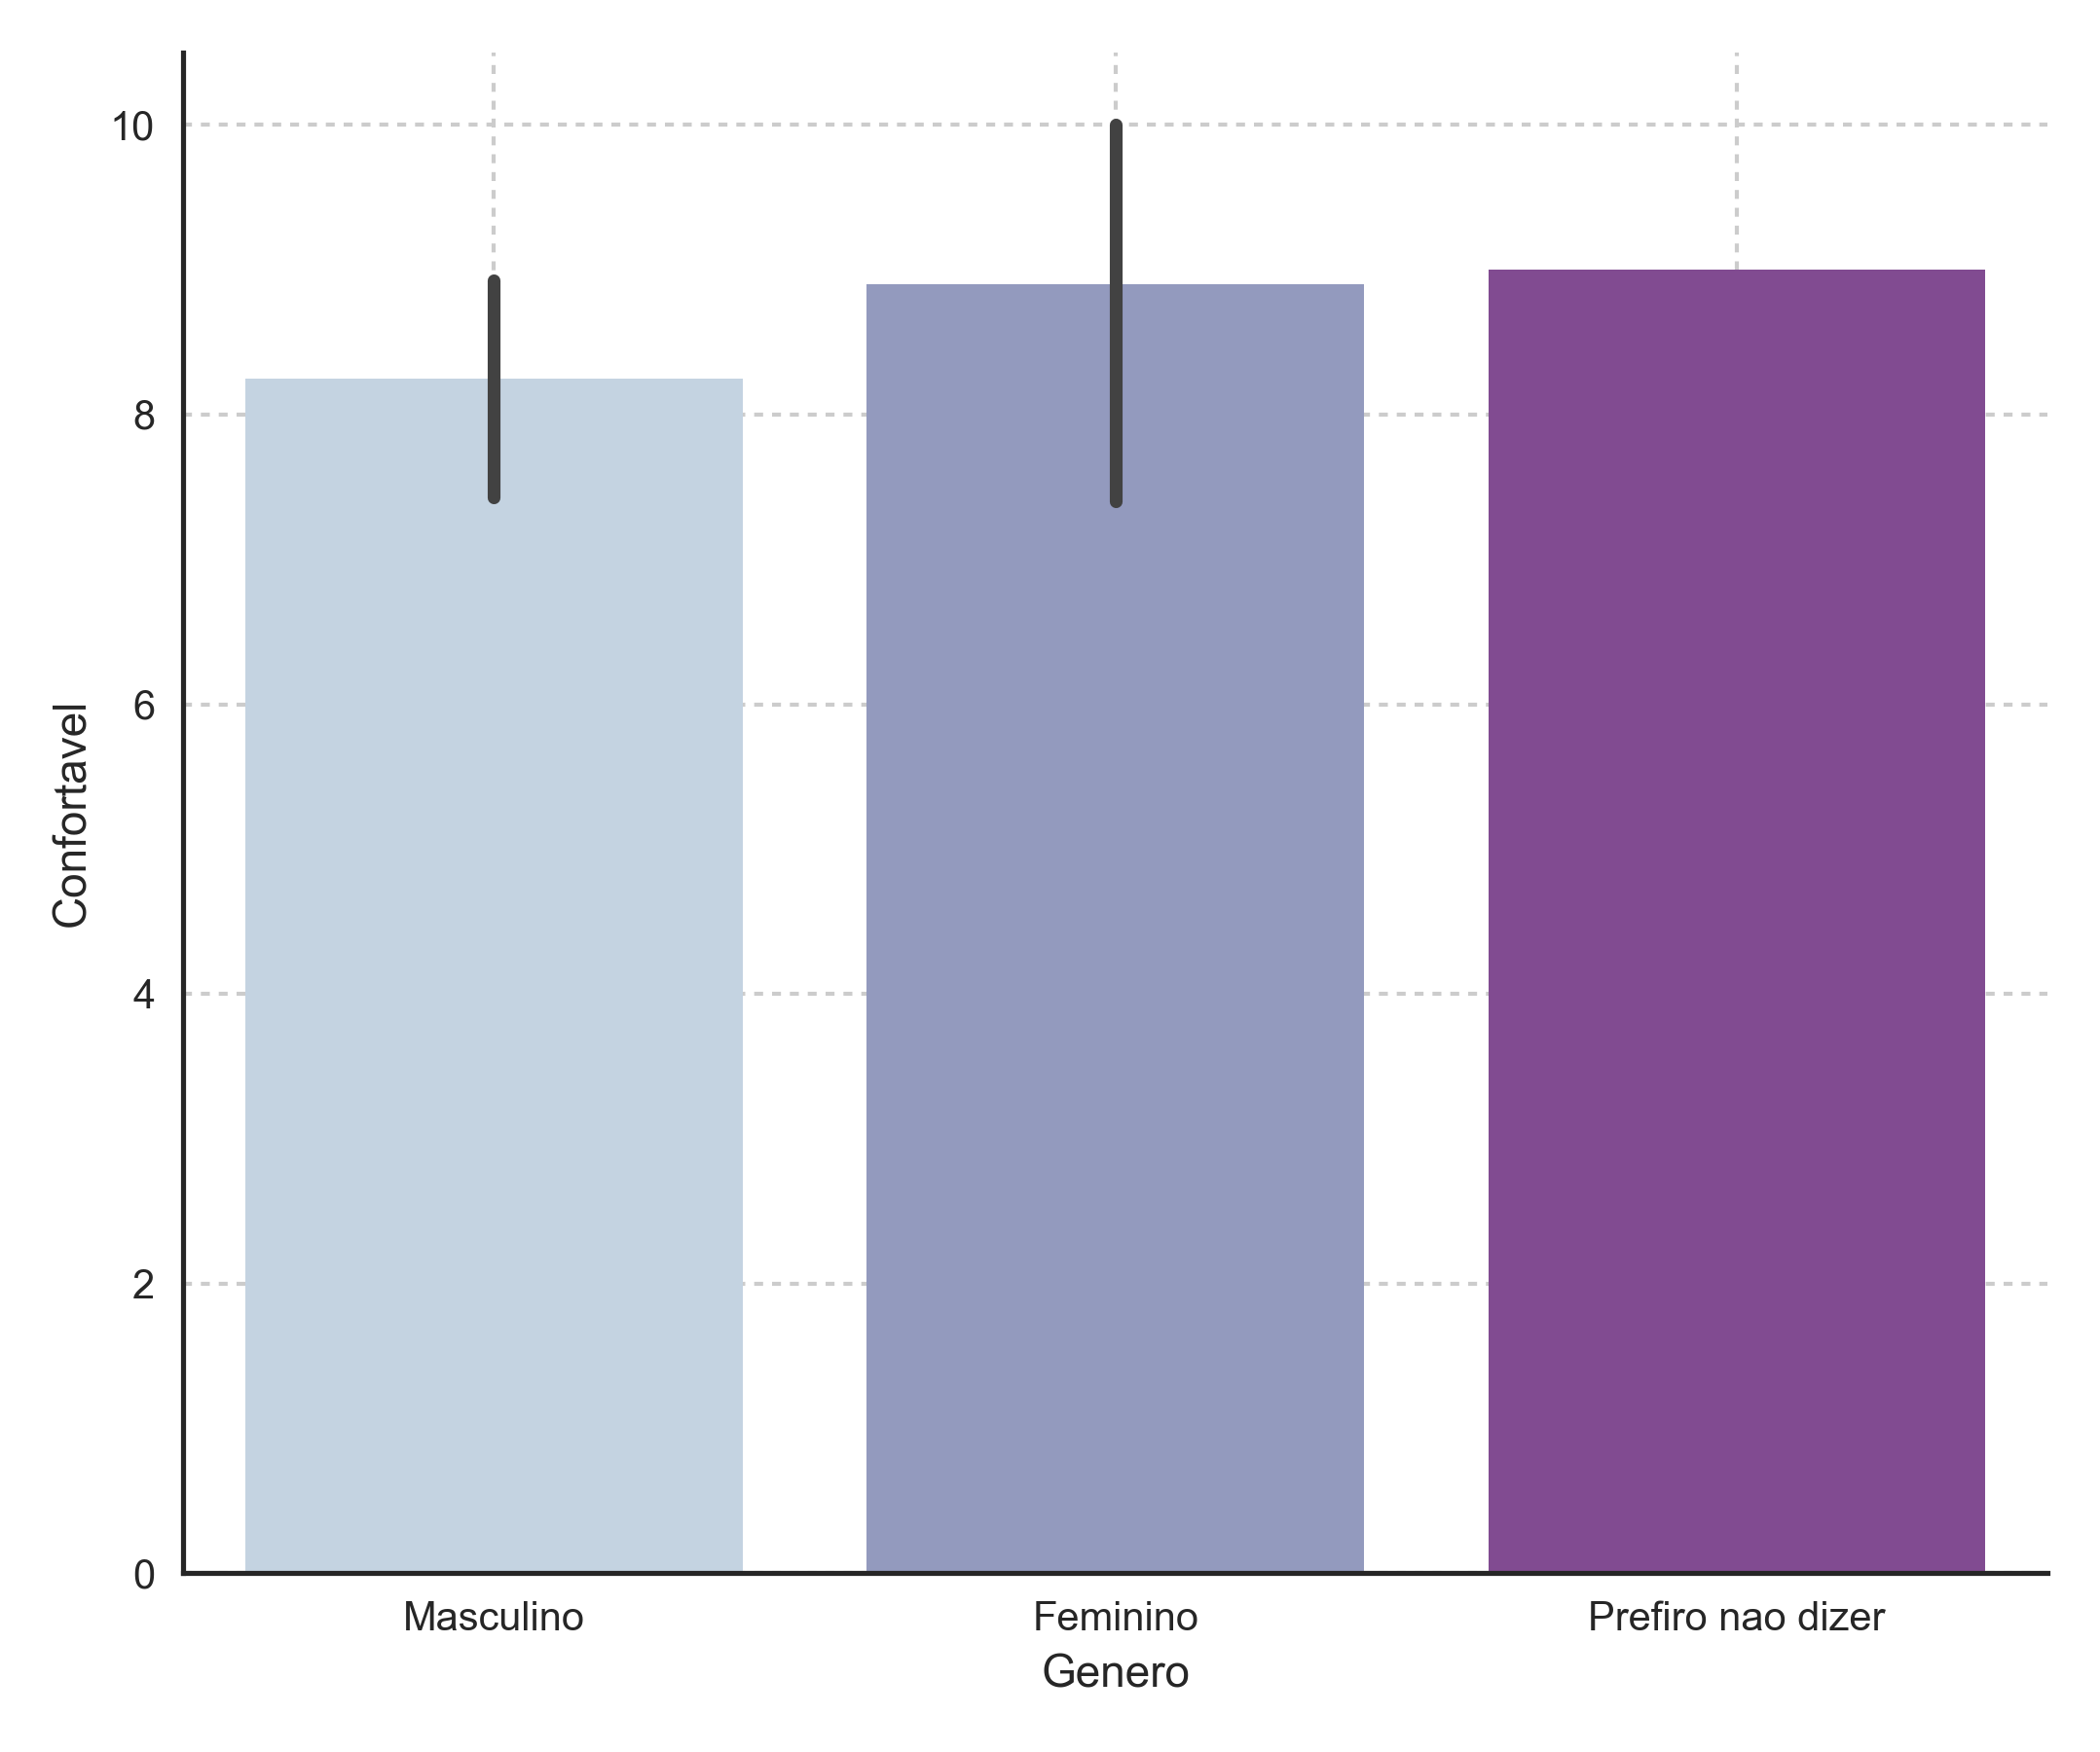
\includegraphics[width=\textwidth]{conforto_genero.png}
		\smallcaption{Fonte: O autor.}
		\label{fig:confortogenero}
	\end{minipage}
\end{figure}

Pode-se observar na figura~\ref{fig:confortogenero} que houve um equilíbrio entre os gêneros com relação ao conforto na aproximação do robô. Na média os homens ficaram 8.25 confortável na escala Likert, com o desvio padrão de 1.9933. As mulheres tiveram a média 8.9 e o desvio padrão em 2.0224. Isso ocorreu em grande parte devido a exibição das expressões faciais do robô, de acordo com o observado durante os testes pelo especialista e conferência dos videos gravados durante a seção. Os participantes do gênero feminino acolheram o robô como uma criança ou pessoa meiga se aproximando dela, conforme comentado em entrevista após os testes pelos participantes do gênero. Outra variável que é comparada é a idade dos partipantes com o nível de conforto, apresentado na figura~\ref{fig:confortoidade}.

\begin{figure}[ht!]
	\centering
	\begin{minipage}{0.65\textwidth}
		\caption{Conforto por idade.}
		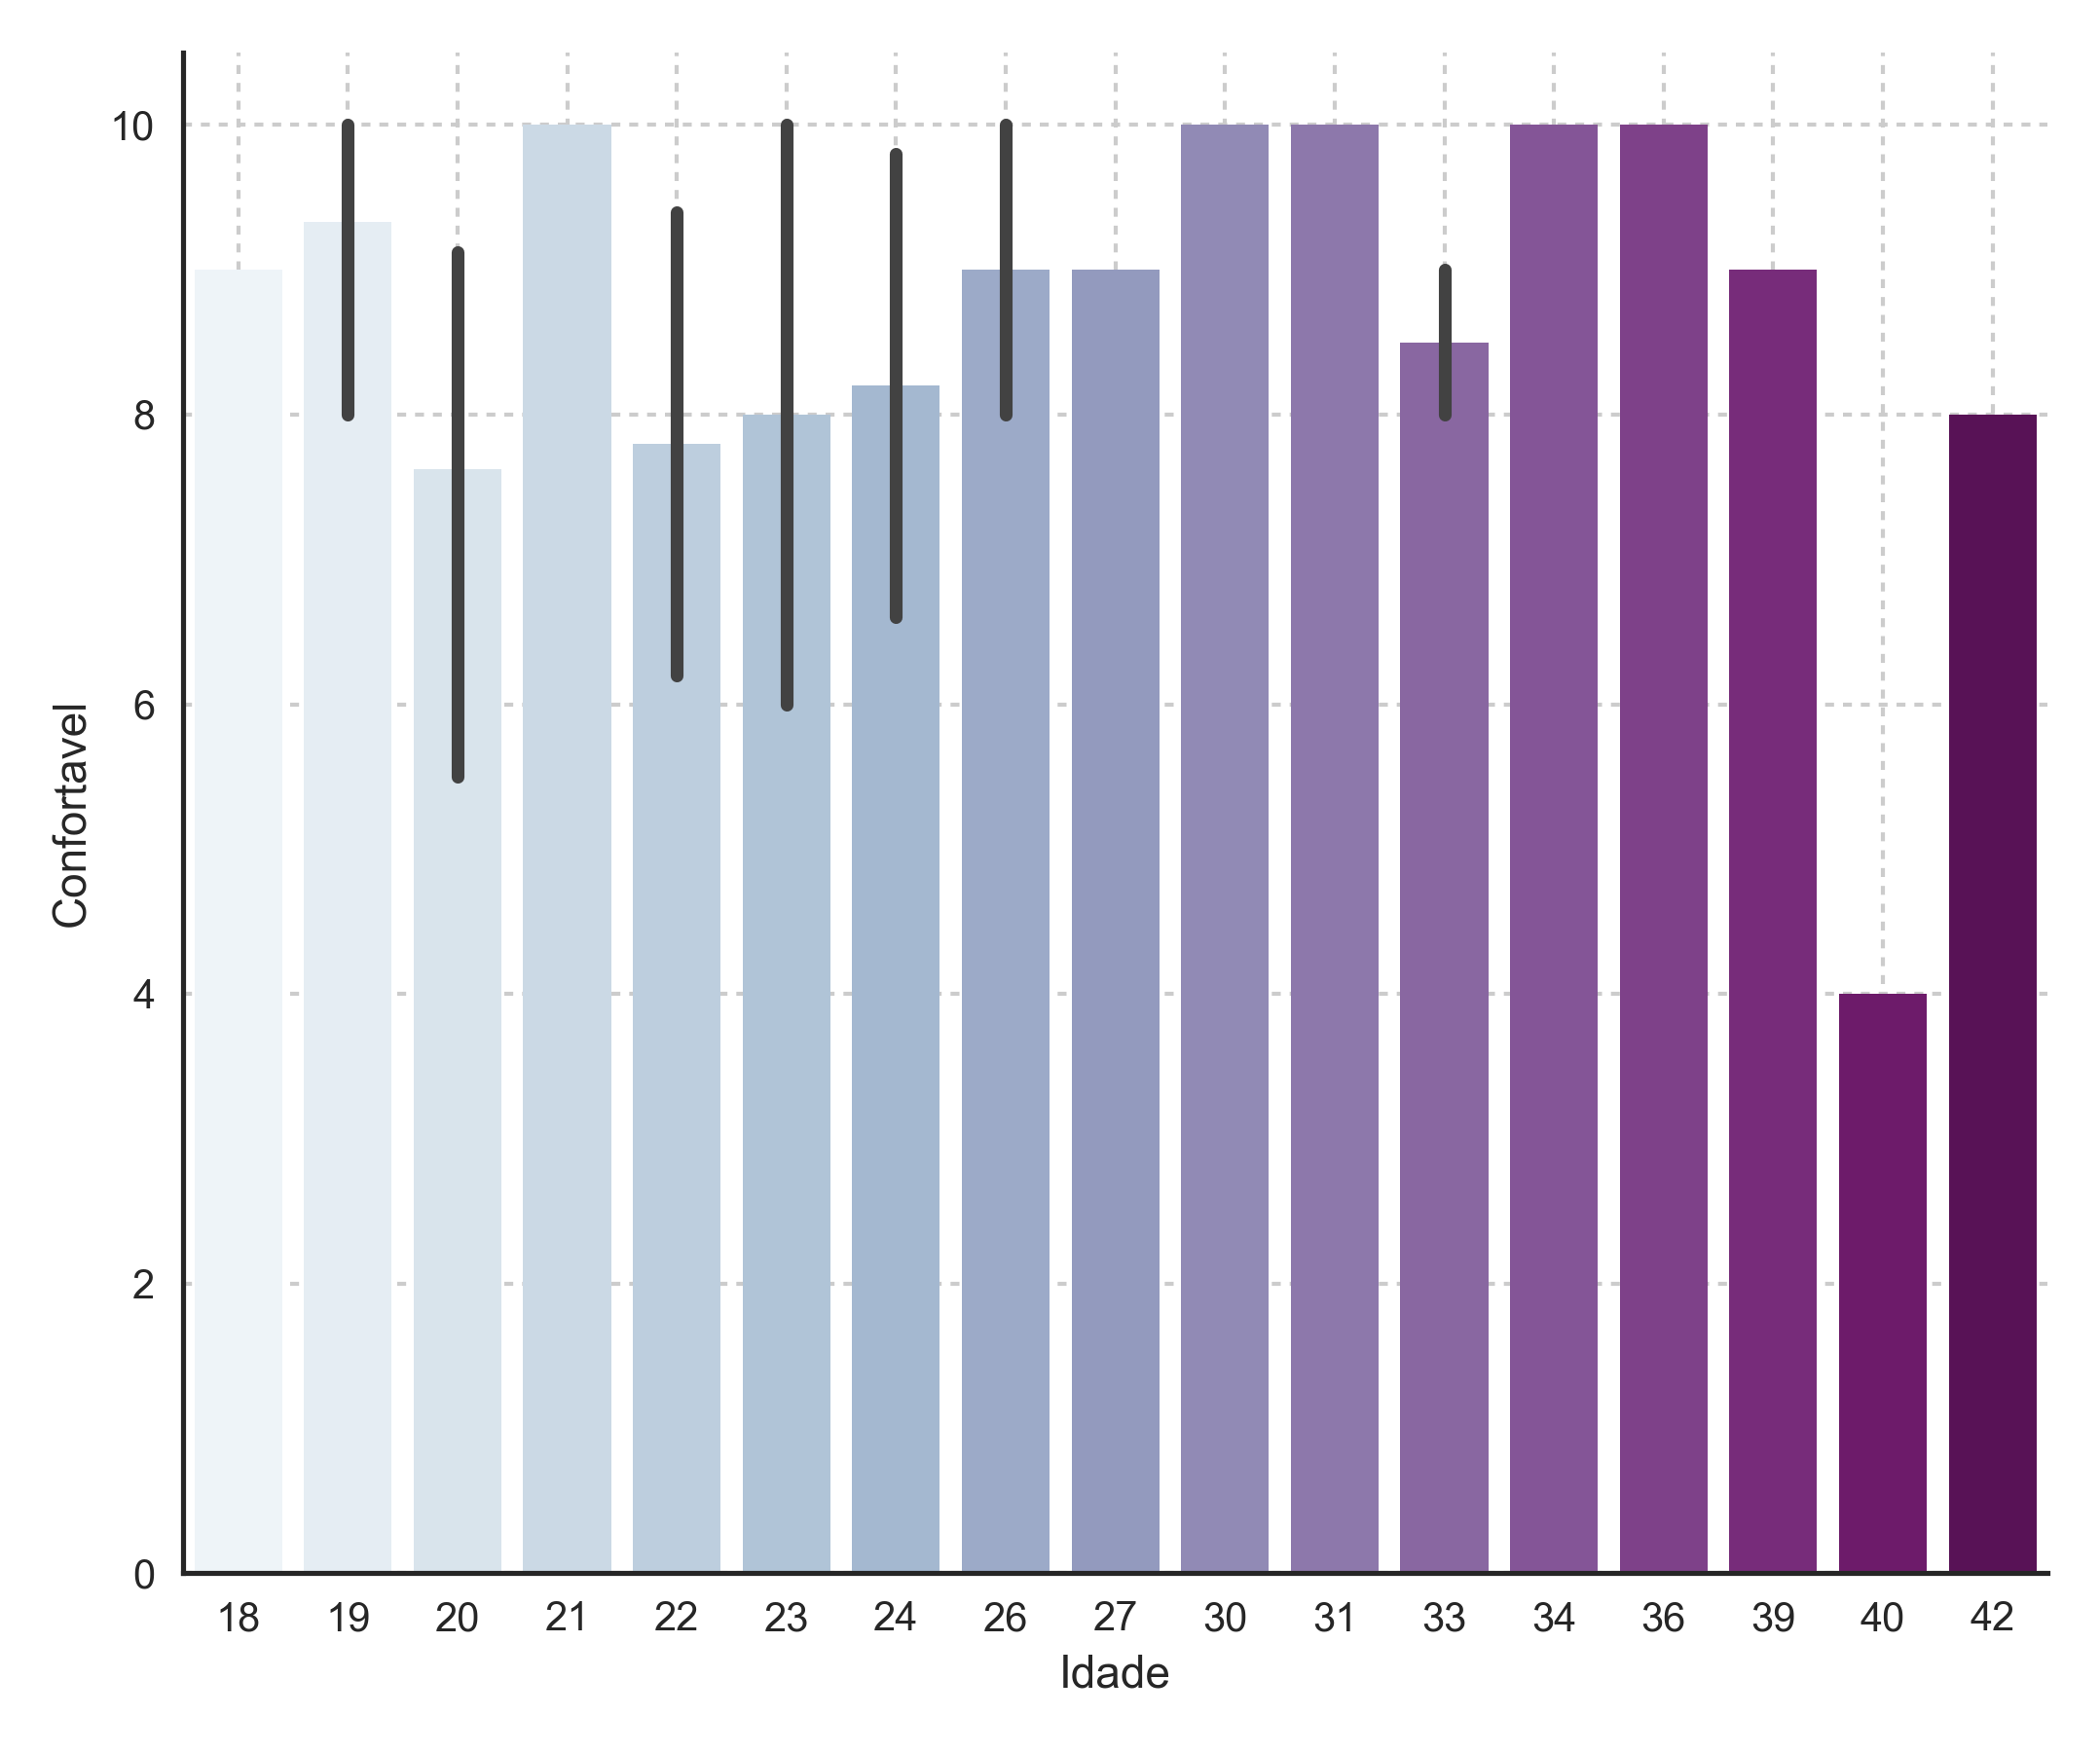
\includegraphics[width=\textwidth]{conforto_idade.png}
		\smallcaption{Fonte: O autor.}
		\label{fig:confortoidade}
	\end{minipage}
\end{figure}

Dois participantes apresentaram um nível de desconforto, mais elevado que os demais participantes, na aproximação do robô. Um participante apresentou a idade de 20 anos e outro de 40 anos. Foram os que ficaram mais desconfortáveis com o robô, como observado na figura~\ref{fig:confortoidade}. Os demais demonstraram-se confortavéis com o robô na aproximação.

Na figura~\ref{fig:confortoposicao} é apresentada a relação entre o conforto do participante e a posição dele durante a interação, sentado ou em pé.

\begin{figure}[ht!]
	\centering
	\begin{minipage}{0.65\textwidth}
		\caption{Conforto por posição de interação.}
		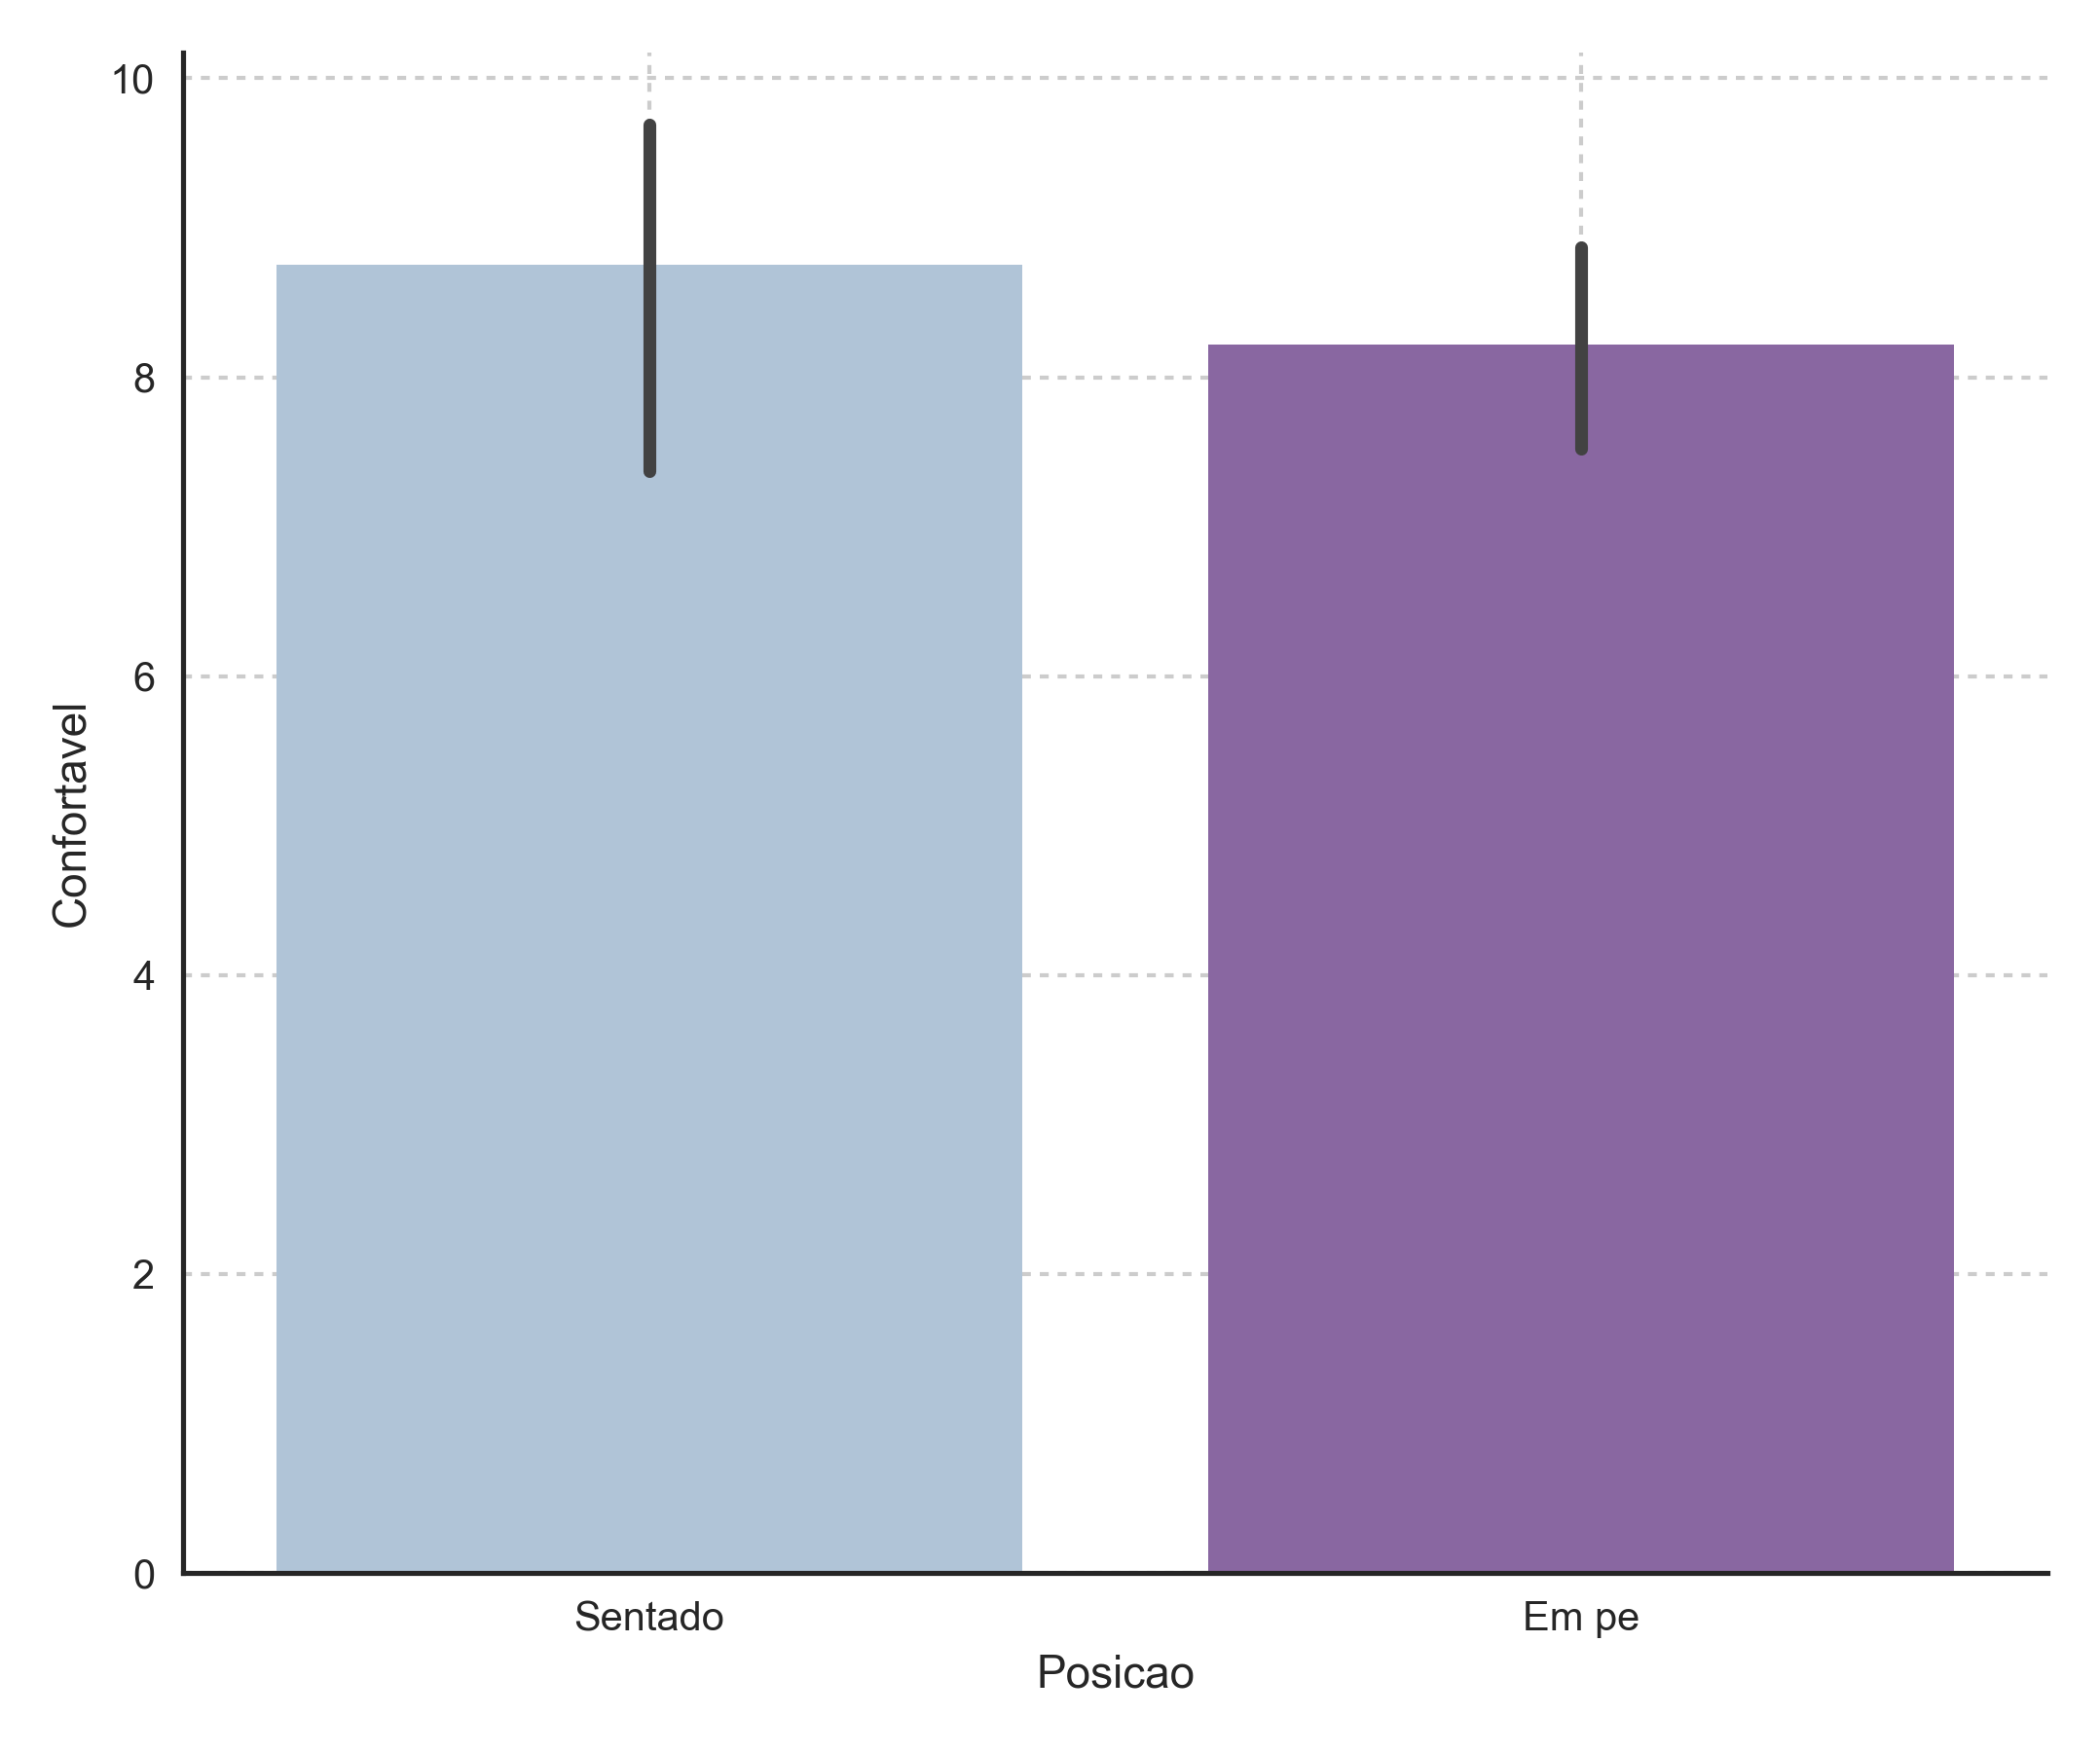
\includegraphics[width=\textwidth]{conforto_posicao.png}
		\smallcaption{Fonte: O autor.}
		\label{fig:confortoposicao}
	\end{minipage}
\end{figure}

É observado na figura~\ref{fig:confortoposicao} o oposto observado na competição da RoboCup@Home. Na competição, as pessoas sentadas sentiram-se com maior desconforto. Nos testes, as pessoas que estavam sentadas durante a interação com o robô sentiram-se mais confortavéis do que as pessoas que estavam em pé. Na média as pessoas em pé apresentaram um grau de conforto igual a 8.2174 e desvio padrão de 1.6407. Já as pessoas sentadas mantiveram uma média de 8.75 de grau de conforto, com desvio padrão 2.3848. Esse fenômeno ocorreu, pois o robô tocou no braço e barriga de alguns participantes que estavam em pé quando esticou o manipulador para chamar a atenção deles. O fenômeno do toque é um ponto de atenção que deve ser tratado em uma nova iteração do ciclo de desenvolvimento do projeto, como uma futura evolução no controle do manipulador. Por último, é apresentado na figura~\ref{fig:confortosociavel} o nível de conforto dos participantes, dado a sua declaração de sociável ou não.

\begin{figure}[ht!]
	\centering
	\begin{minipage}{0.65\textwidth}
		\caption{Conforto por declaração de sociável.}
		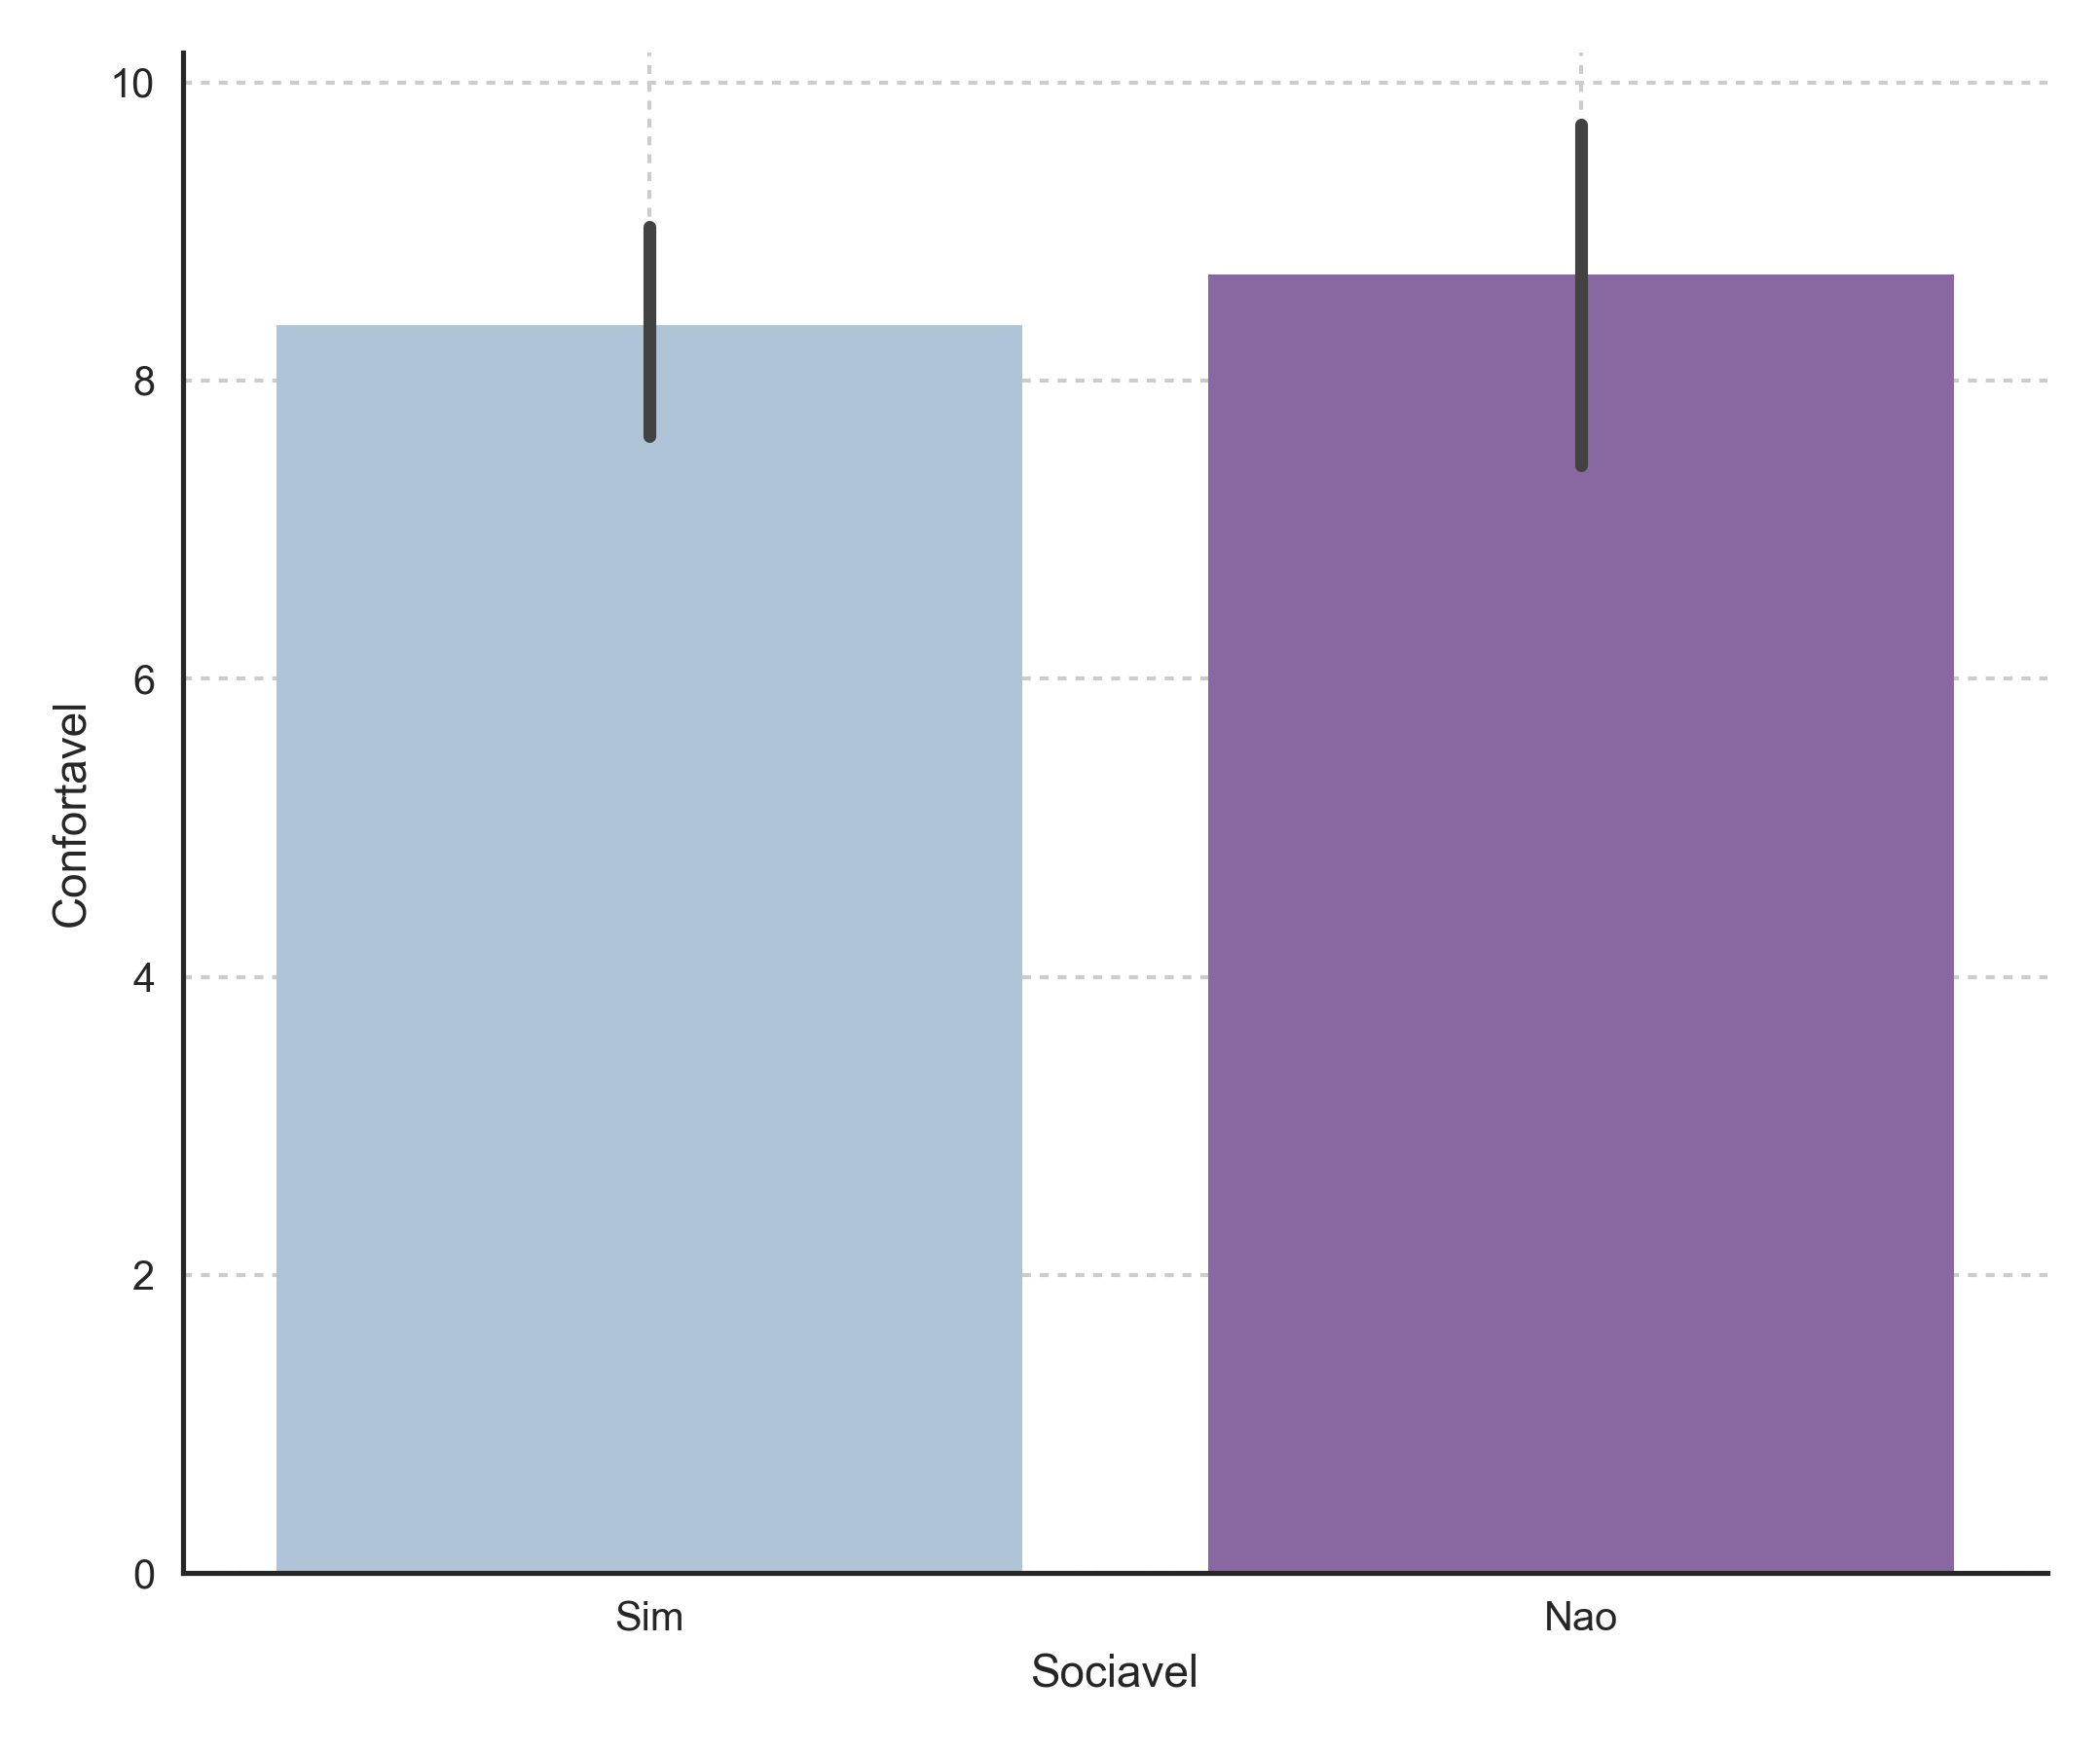
\includegraphics[width=\textwidth]{conforto_sociavel.png}
		\smallcaption{Fonte: O autor.}
		\label{fig:confortosociavel}
	\end{minipage}
\end{figure}

Nessa análise feita através da figura~\ref{fig:confortosociavel}, as pessoas declaradas como não sociáveis, foram as pessoas que mais se sentiram confortáveis durante toda a aproximação do robô. Na média uma pessoa sociável apresentou um grau de conforto de 8.375, com desvio padrão de 2.0729. Já a pessoa não sociável apresentou 8.7143 na média, com desvio padrão de 1.5779. É um ponto interessante, pois se observar, as pessoas sociáveis deveriam estar mais confortável e abertas a novas experiências.

Algumas situações durante o cenário de interação causaram medo, como por exemplo, o manipulador tocado o participante. E na mesma situação, o usuário ficou confortável ao ver a expressão facial amigável do robô, esboçando um sorriso. Assim, a mesma análise para o conforto do usuário, foi realizada para a declaração de medo. Na escala da pergunta sobre medo do robô, o menor valor corresponde a totalmente com medo (valor 0 da escala) e o maior corresponde a totalmente sem medo (valor 10 da escala). A figura~\ref{fig:medogenero} apresenta a relação entre o medo e o gênero do participante.

\begin{figure}[ht!]
	\centering
	\begin{minipage}{0.65\textwidth}
		\caption{Medo por gênero.}
		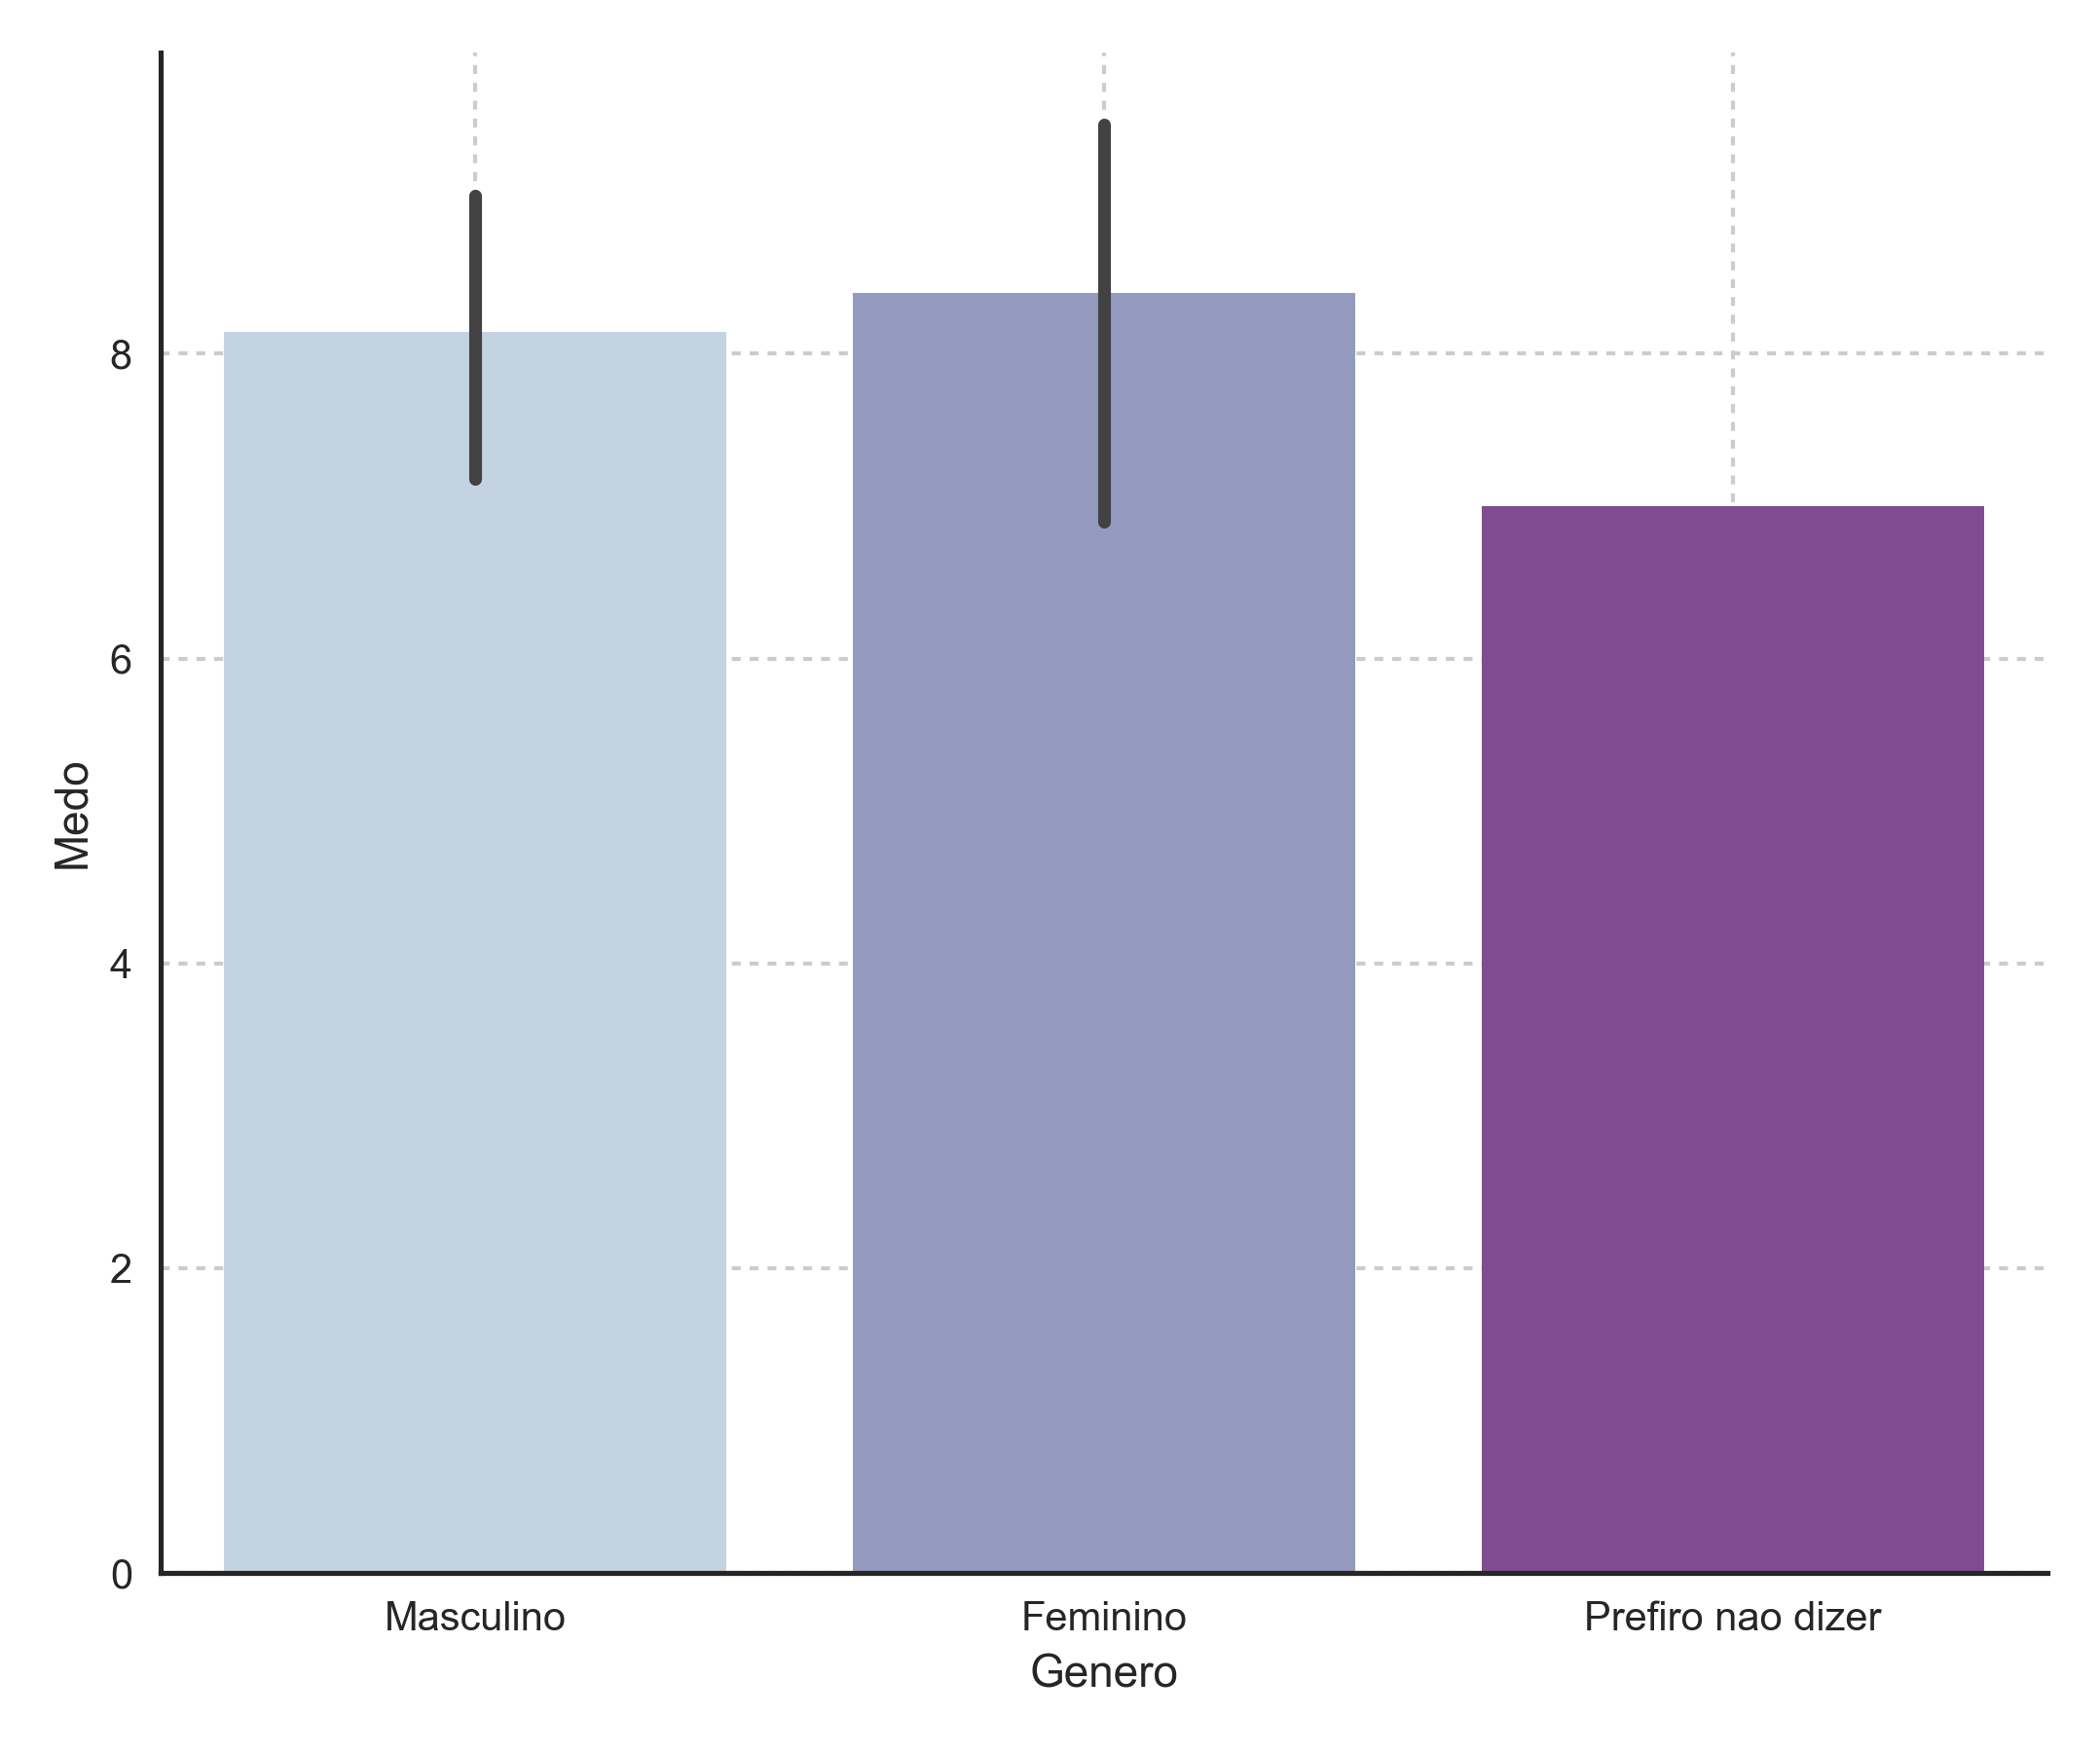
\includegraphics[width=\textwidth]{medo_genero.png}
		\smallcaption{Fonte: O autor.}
		\label{fig:medogenero}
	\end{minipage}
\end{figure}

Para a relação de medo e gênero, o que observa-se na figura~\ref{fig:medogenero} é que o gênero feminino sentiu menos medo. Porém, a diferença não foi tão grande assim. Na média as mulheres tiveram 8.4 graus, com desvio padrão de 2.1071. Enquanto isso, os homens ficaram com a média de 8.1429, desvio padrão de 2.6010. Era esperado este resultado, devido as observações sobre o conforto do usuário, apesar dessa relação nem sempre ser diretamente proporcional. Na sequência é feita a análise com base na relação medo e idade, demonstrada na figura~\ref{fig:medoidade}.

\begin{figure}[ht!]
	\centering
	\begin{minipage}{0.65\textwidth}
		\caption{Medo por idade.}
		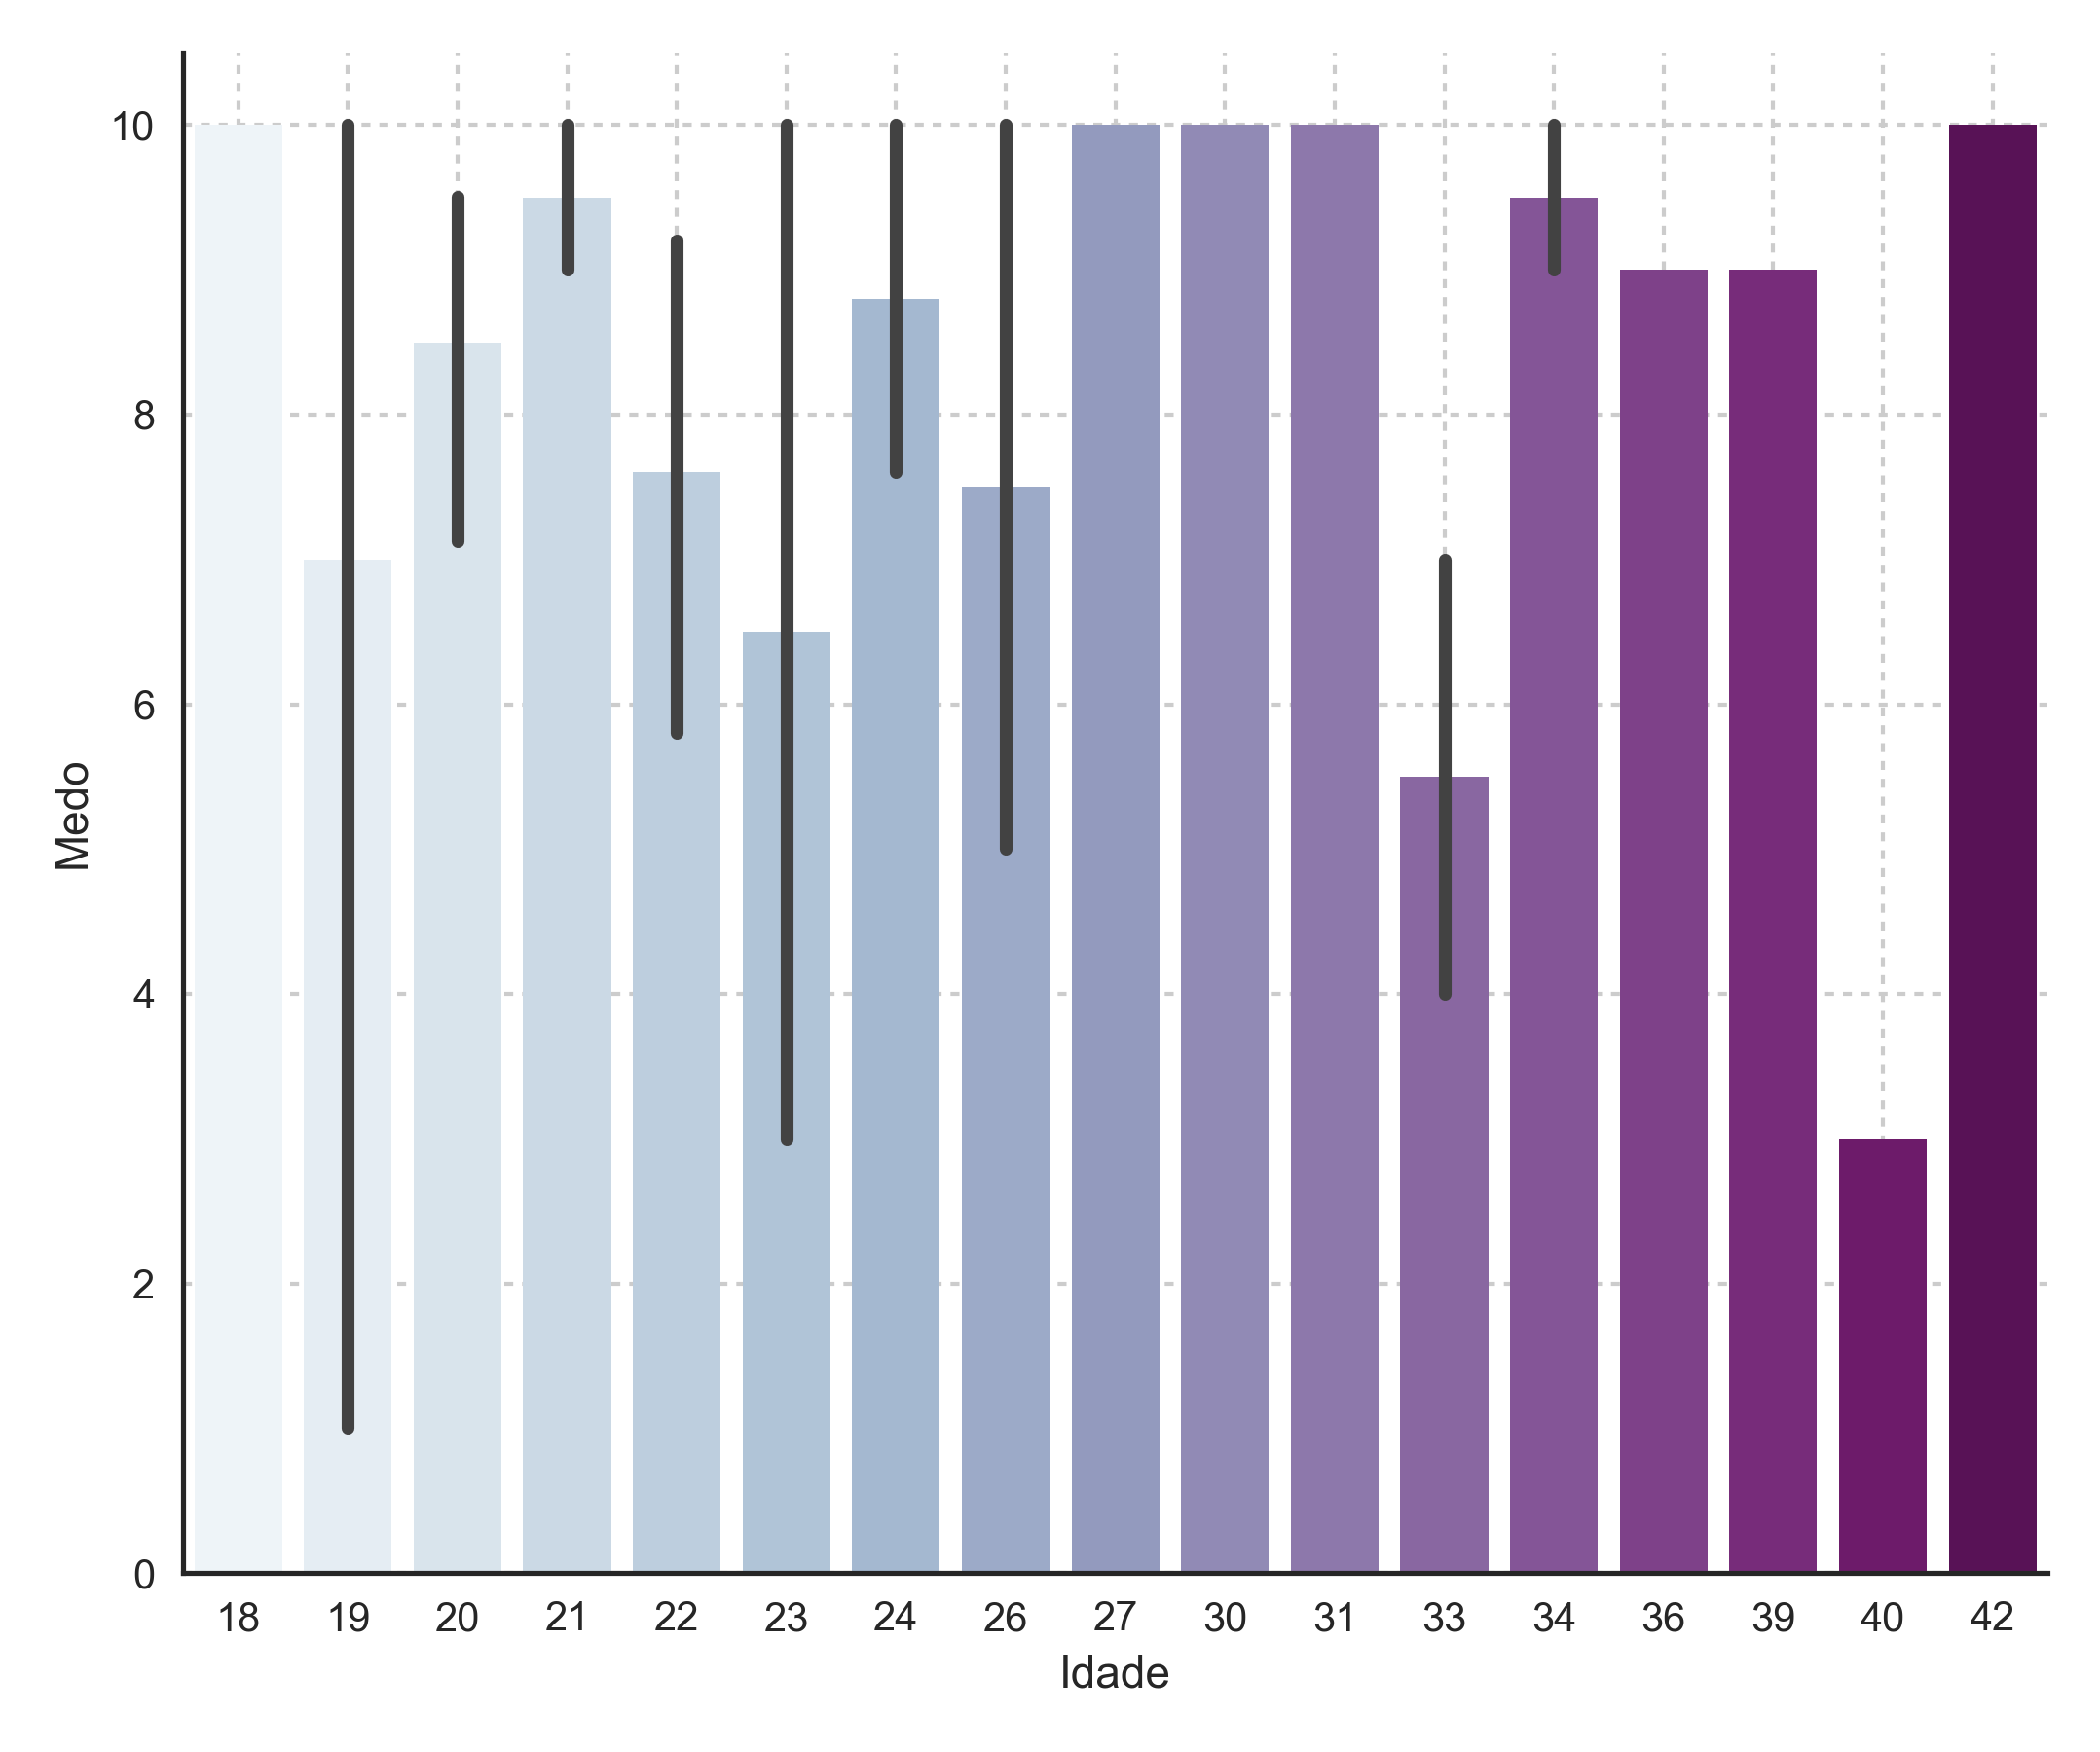
\includegraphics[width=\textwidth]{medo_idade.png}
		\smallcaption{Fonte: O autor.}
		\label{fig:medoidade}
	\end{minipage}
\end{figure}

Um participante na faixa etária de 40 anos, apresentou o maior índice de medo, conforme figura~\ref{fig:medoidade}. Os participantes com 19 anos também apresentam um índice baixo, que indica medo do participante. Isso ocorreu, pois com o comportamento invasivo do robô ao aproximar, a garra deixou o participante assustado. Outro ponto levantado foi que o robô ao se movimentar faz muito barulho, devido ao novo conjunto de rodas omnidirecionais.

A figura~\ref{fig:medoposicao} compara a relação do medo declarado do usuário contra a posição dele durante a navegação do robô.

\begin{figure}[ht!]
	\centering
	\begin{minipage}{0.65\textwidth}
		\caption{Medo por posição de interação.}
		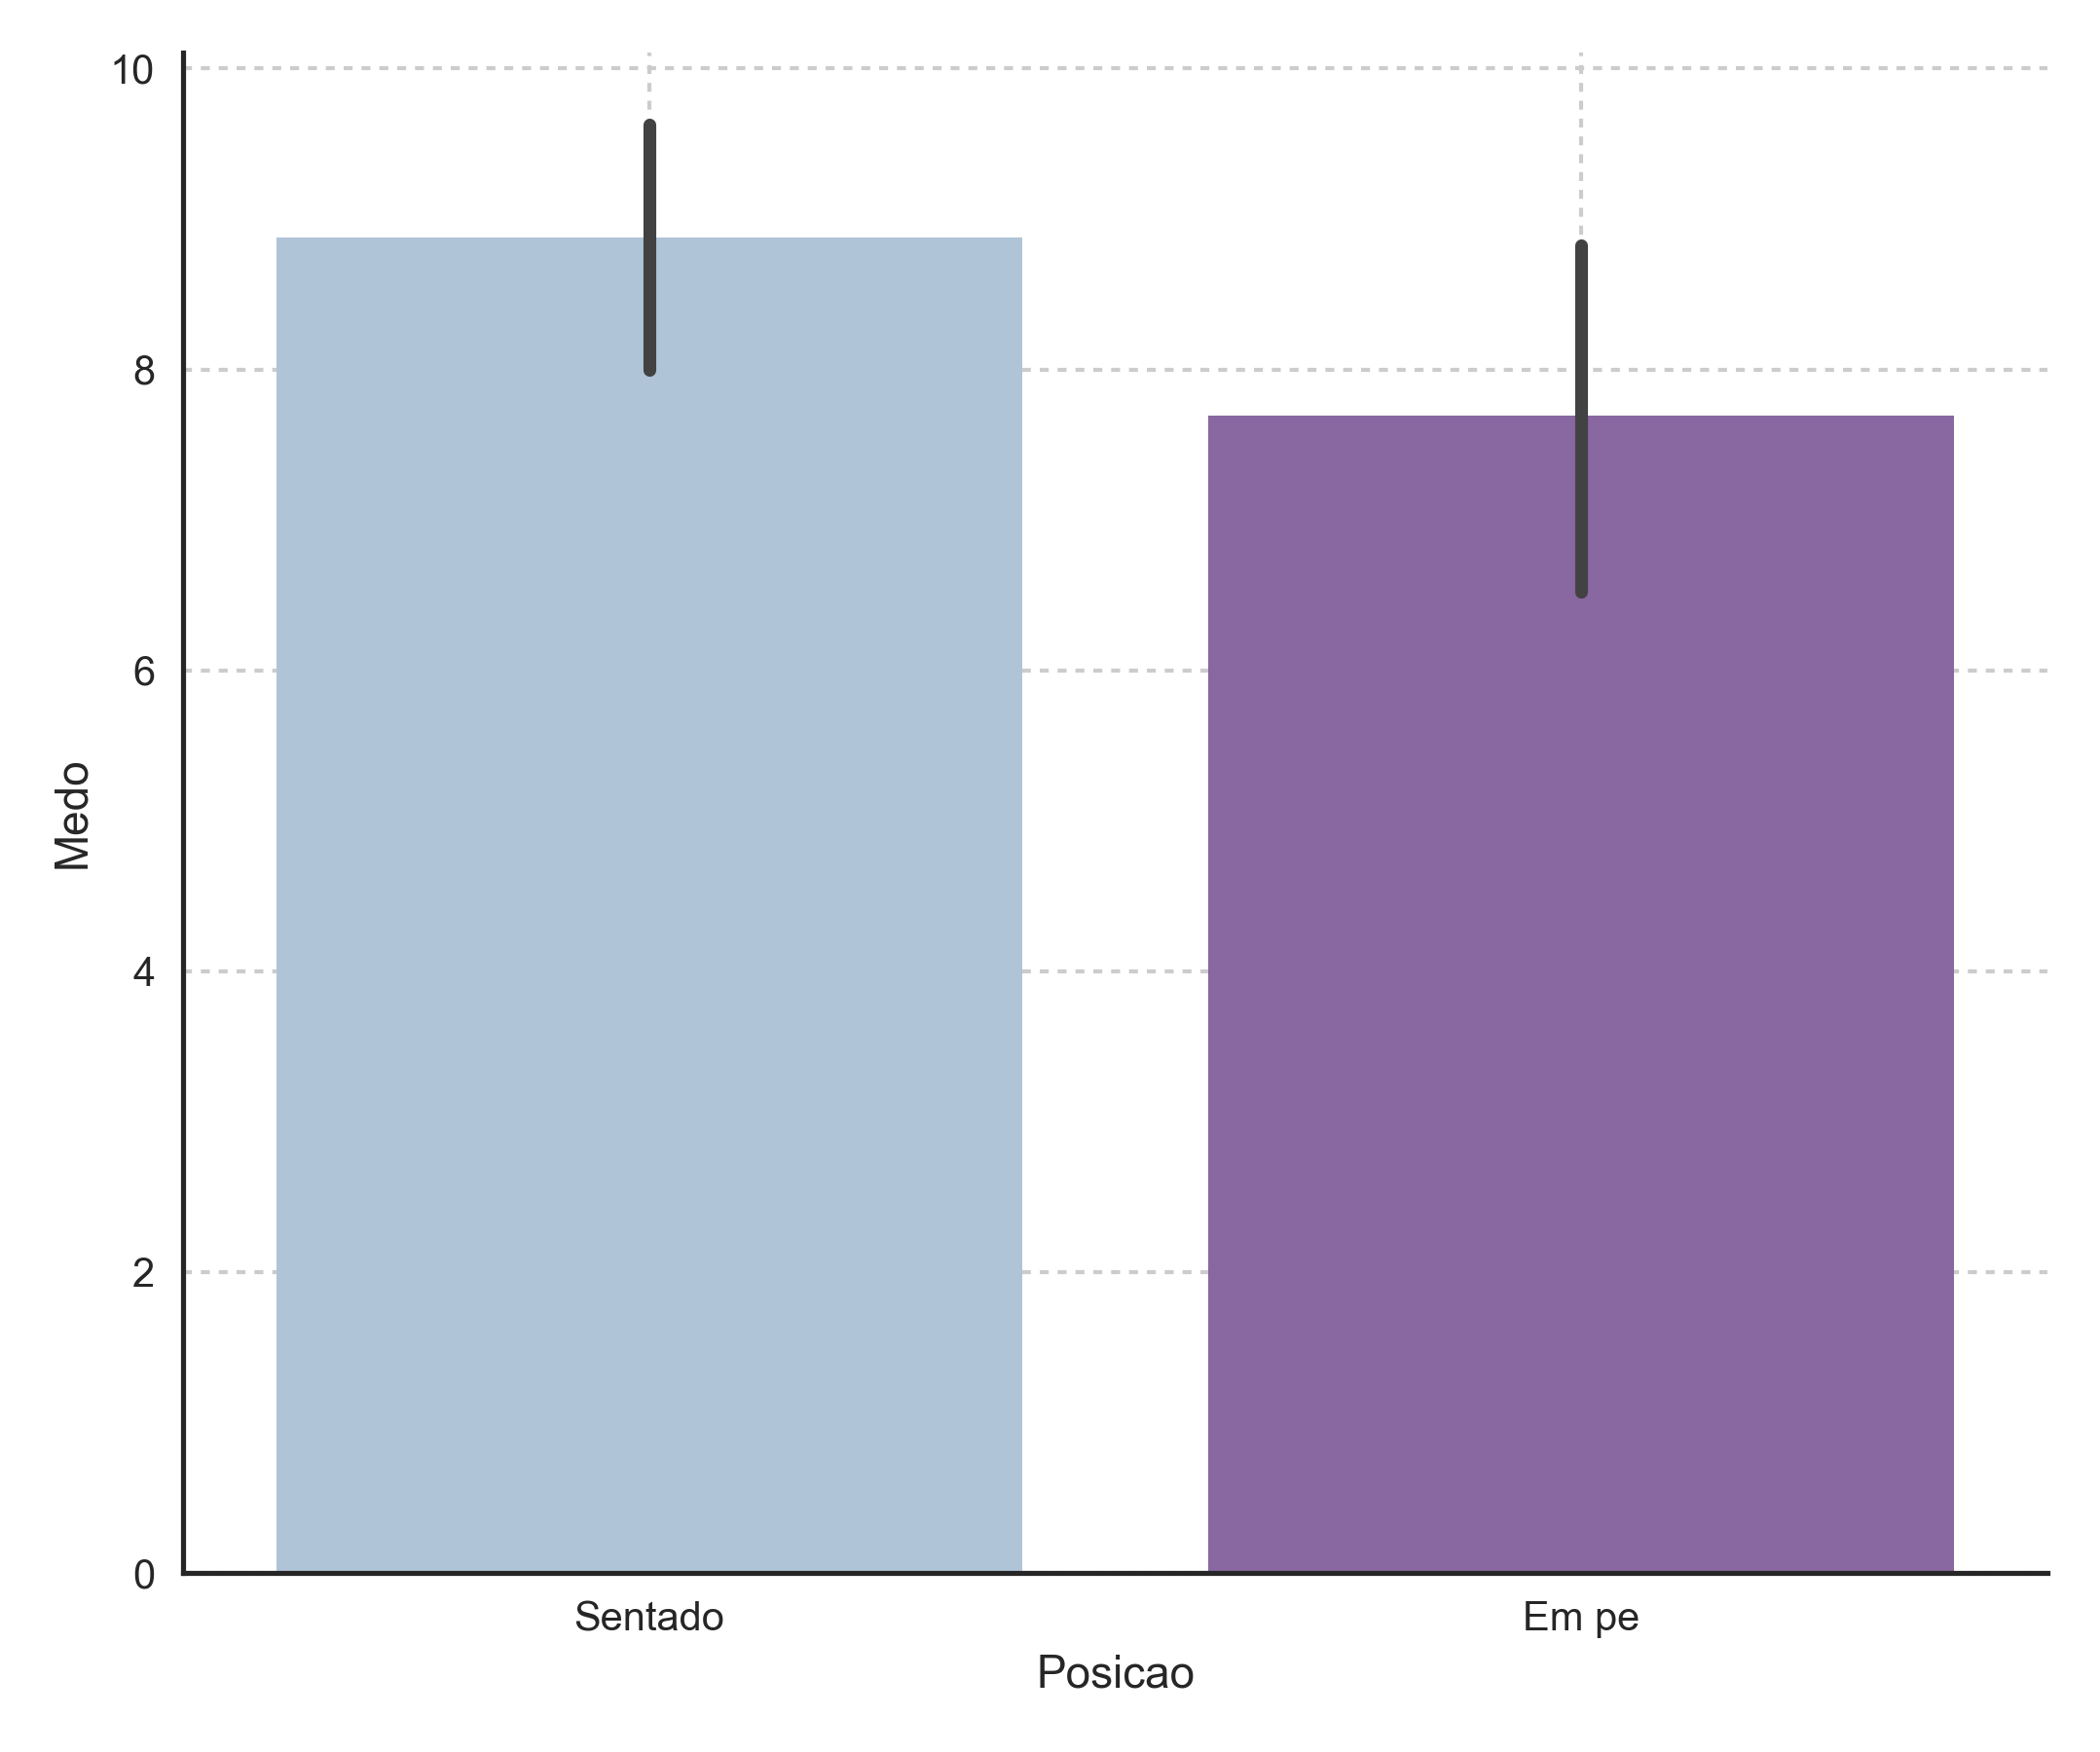
\includegraphics[width=\textwidth]{medo_posicao.png}
		\smallcaption{Fonte: O autor.}
		\label{fig:medoposicao}
	\end{minipage}
\end{figure}

Assim como em relação ao conforto do usuário, os participantes que sentiram mais medo do robô estavam em pé. Os participantes sentados apresentaram uma média de 8.8750, com desvio padrão de 1.6910. Comparando, os participantes em pé tiveram 7.6957 de média e um desvio padrão de 2.7731. O manipulador é um ponto de atenção na interação, principalmente quando está dentro do espaço social da pessoa. Os maiores índices de medo ocorreram por que o robô encostou o manipulador na pessoa, sem nenhum aviso prévio. As pessoas mais sociáveis sentiram menos medo que as menos sociáveis, como apresenta na figura~\ref{fig:medosociavel}. Na média as pessoas sociáveis apresentam 8.4688 contra 6.8571 das pessoas não sociáveis. Os desvios padrão apresentaram os valores 2.0461 e 3.5225, respectivamente.

\begin{figure}[ht!]
	\centering
	\begin{minipage}{0.65\textwidth}
		\caption{Medo por declaração de sociável.}
		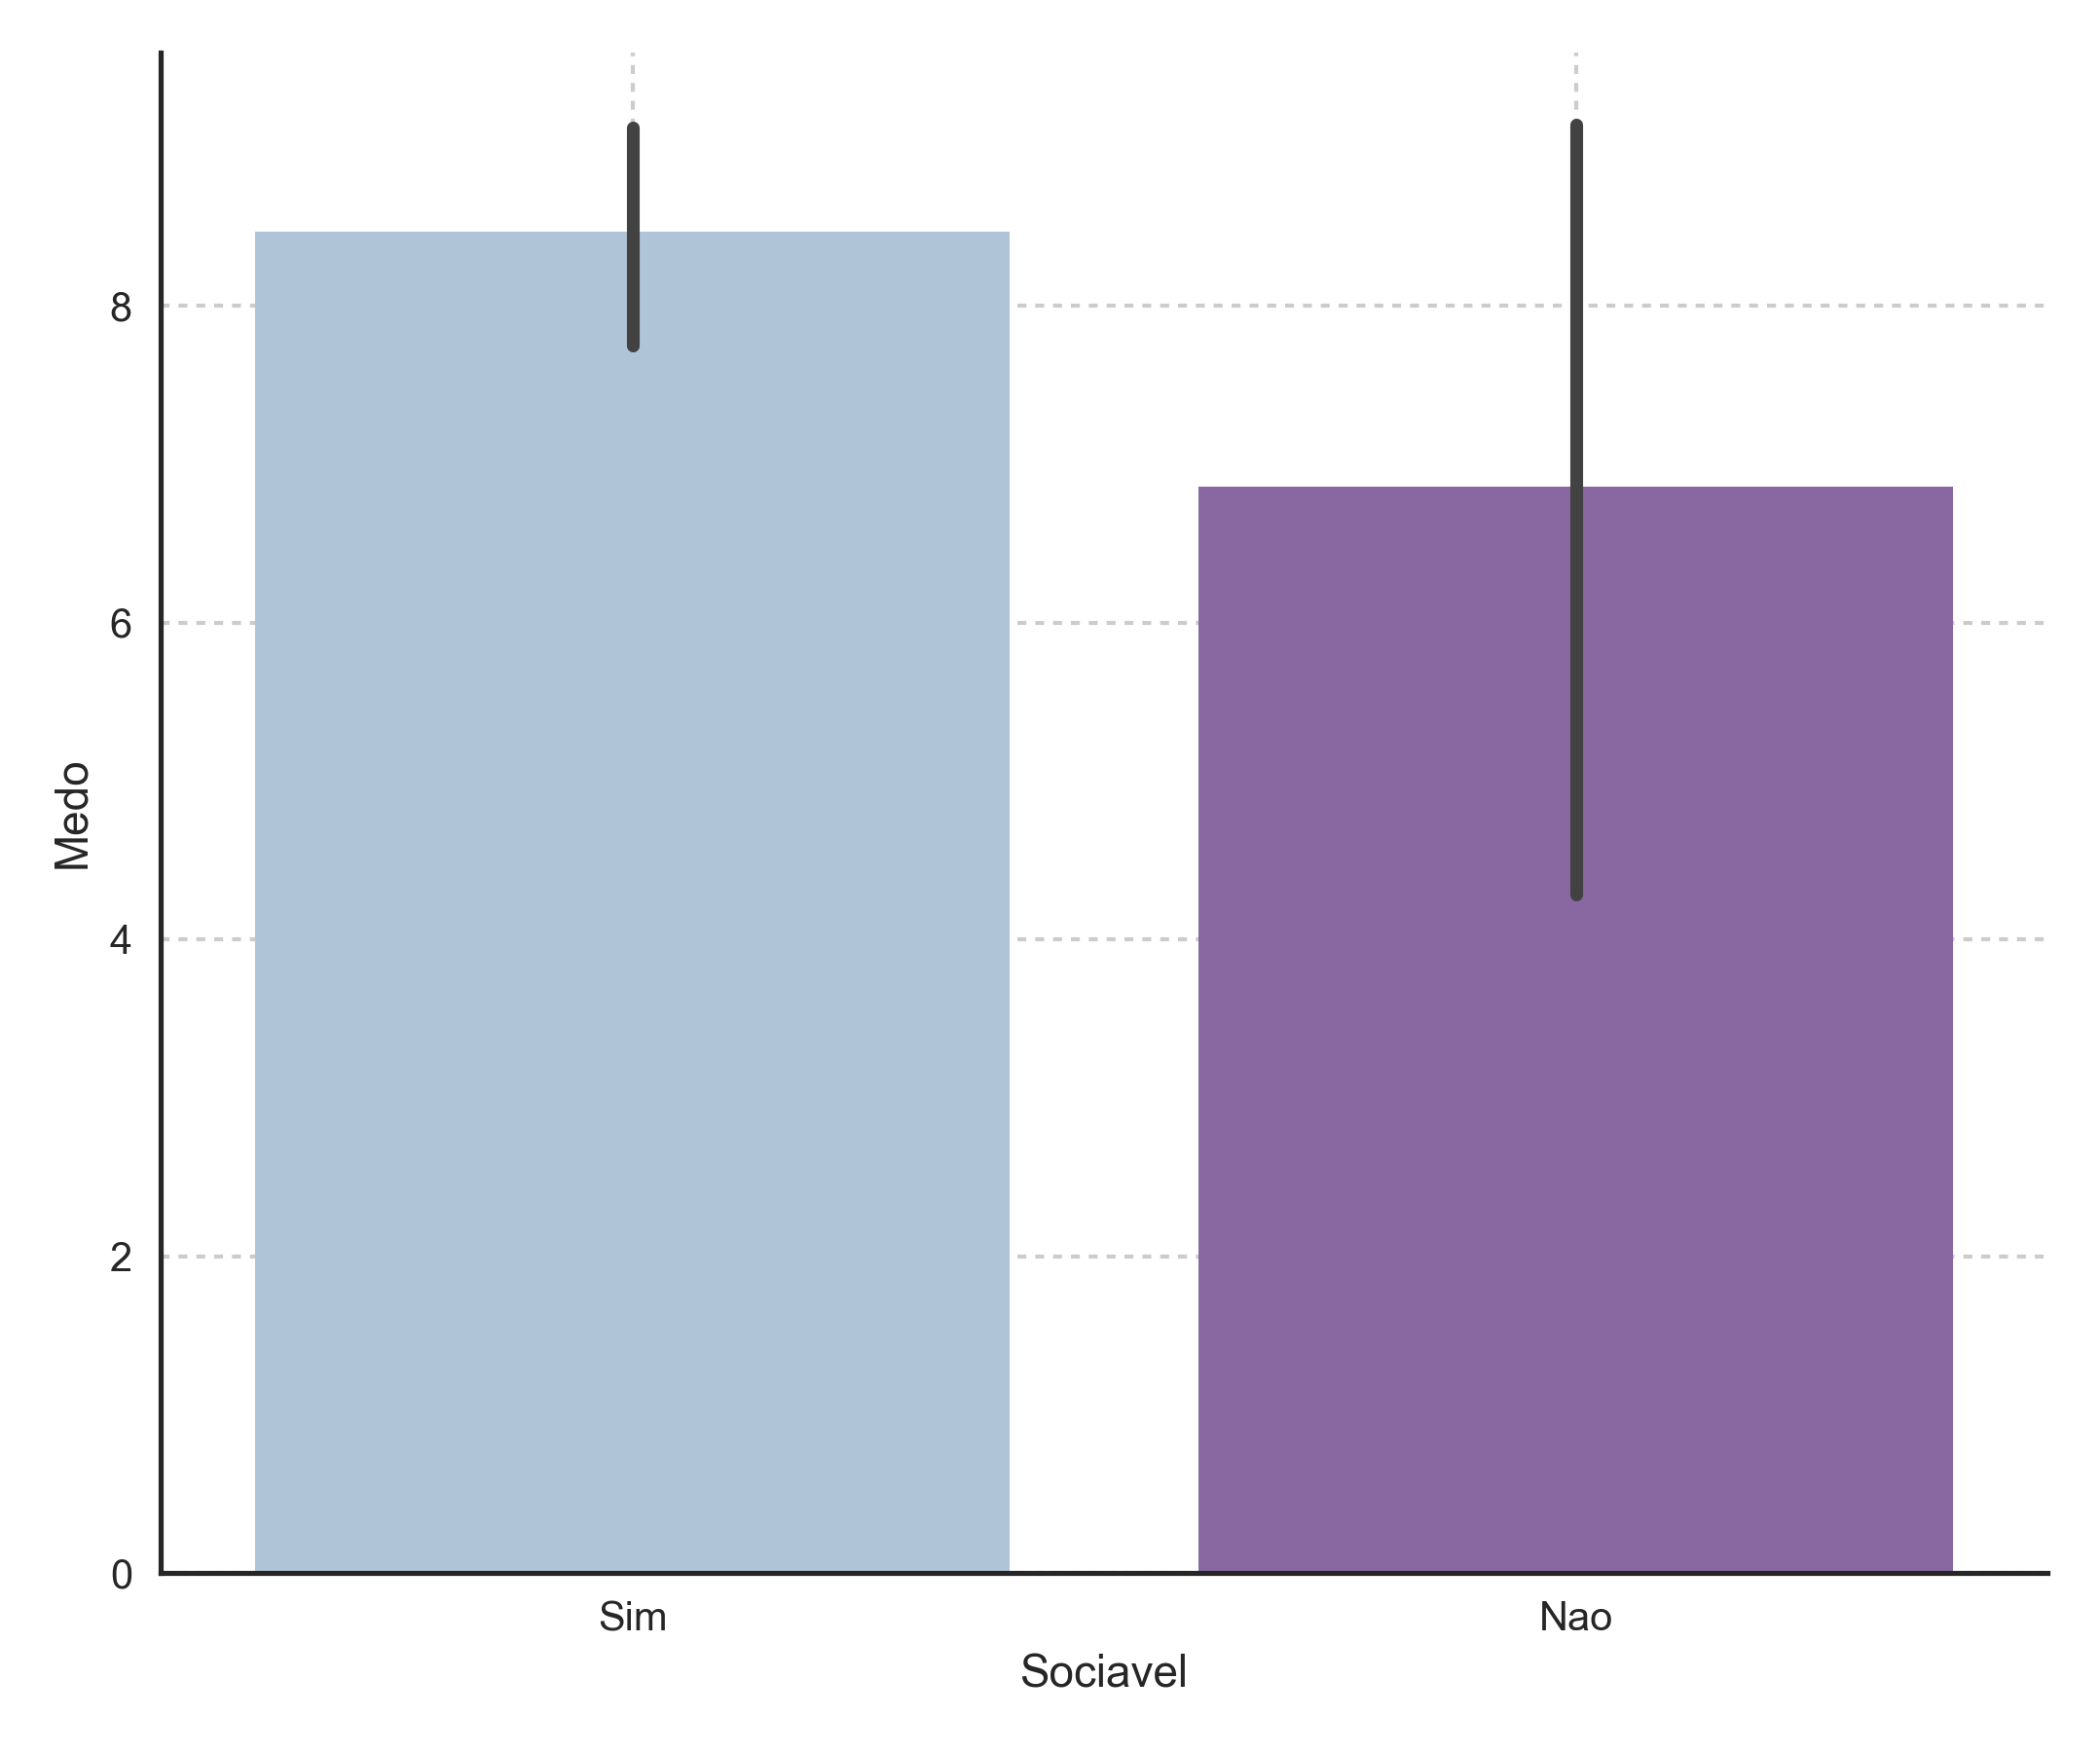
\includegraphics[width=\textwidth]{medo_sociavel.png}
		\smallcaption{Fonte: O autor.}
		\label{fig:medosociavel}
	\end{minipage}
\end{figure}

Após as análises gerais sobre as informações coletadas, é realizado o processo para obter os grupos de perfis de usuários, conforme seção~\ref{sec:criacaopersonas}. Para obter os grupos de perfis, utilizou-se o algoritmo de agrupamento por similaridade QG-SIM. Foram testados três valores Q, que determinam a similaridade mínima do grupo, para determinar os grupos. Os valores utilizados foram 0.6, 0.7 e 0.8. O valor 0.6 resultou em 3 grupos, porém um dos grupos manteve 90\% dos perfis e ou outros 10\% foram distribuídos entre os dois grupos restantes. O valor $Q = 0.6$ apresentou resultado muito generalizado e que não condiz com os perfis que realizaram os testes.

Quando aplicado o valor de 0.8 de similaridade para o algoritmo, 7 grupos foram encontrados. Nessa situação, os grupos ficaram bem específicos, sendo que 4 dos 7 grupos eram compostos por apenas 1 pessoa. Dessa maneira, é possível comprovar que o resultado gerado é muito especializado. Elevar o grau de similaridade nesse ponto, provavelmente serão encontrados mais grupos com apenas uma pessoa. Esse não é o objetivo da técnica de Personas. Então este resultado também foi desconsiderado.

O valor intermediário, 0.7, foi escolhido. Ele resultou em 5 grupos. Um grupo com 21 perfis, que resultou na Persona Joaquim (vide tabela~\ref{tab:joaquim}). Um grupo com 7 pessoas para Persona Maria Eduarda (vide tabela~\ref{tab:mariaeduarda}). Outro grupo com 9 pessoas deu origem a Persona Alfredo (vide tabela~\ref{tab:alfredo}). As outras duas Personas foram criadas com base em dois grupos de 1 pessoa. Apesar de serem formados por apenas 1 pessoa, algumas características foram totalmente descriminante. A Persona Manuel (vide tabela~\ref{tab:manuel}), por exemplo, não tem acesso, nem conta em redes sociais. E a Persona Danielo (vide tabela~\ref{tab:danielo}) aplicou a nota positiva máxima em todas as situações de interação. Esses fatores foram decisivos para que esses perfis permanecessem isolados em um grupo cada um.

Cada perfil dentro dos grupos mantém uma consistência etnográfica e também sobre a percepção em relação aos comportamentos e ações do robô. As percepções de cada perfil, estão sintetizadas e são apresentadas em grupos de informações similares. Essas informações auxiliaram na descrição de cada Persona. A tabela~\ref{tab:expectativacasa} apresenta um compilado das informações referentes a expectativa de ter um robô em casa, na percepção de cada usuário.

\begin{table}[!ht]
	\caption{Expectativa do robô em casa dos perfis por Persona.}
	\label{tab:expectativacasa}
	\centering
	\begin{tabular}{c | c | c }
        \hline
        \multicolumn{3}{c}{Expectativa do robô em casa?} \\ \hline
        Persona & Observação & Quantidade \\ \hline
        \multirow{7}{*}{Joaquim} & Limpar a casa & 7 \\
        \hhline{~--}
        & Buscar objetos & 1 \\
        \hhline{~--}
        & Cuidar da segurança & 1 \\
        \hhline{~--}
        & Obediência & 4 \\
        \hhline{~--}
        & Afetividade & 4 \\
        \hhline{~--}
        & Naturalidade & 3 \\
        \hhline{~--}
        & Respeito & 3 \\
        \hline
        \multirow{3}{*}{Maria Eduarda} & Realizar tarefas domésticas & 5 \\
        \hhline{~--}
        & Dirigir o carro & 1 \\
        \hhline{~--}
        & Amigável & 1 \\
        \hline
        \multirow{4}{*}{Alfredo} & Realizar tarefas domésticas & 5 \\
        \hhline{~--}
        & Comandos de voz & 2 \\
        \hhline{~--}
        & Obediência & 2 \\
        \hline
        Danielo & Realizar tarefas domésticas & 1 \\
        \hline
        Manuel & Atender necessidades & 1 \\
        \hline
    \end{tabular}
    \smallcaption{Fonte: O autor.}
\end{table}

A pergunta da expectativa do robô em casa foi realizada antes da interação com o robô. Com base nas respostas pode-se perceber que as pessoas, no geral, enxergam os robôs como ferramentas. Essa percepção muda após a interação e a demonstração das habilidades dos robôs. Em alguns casos, a mudança de opinião é nítida, onde comentários como ``ele faz tudo isso sozinho'' são mencionados durante o teste, ou quando o usuário diz que imagina robôs apenas na linha de produção de fábricas e montadores. Outra questão discutida antes da interação com o robô é a expectativa sobre o papel dele, em relação ao ambiente de trabalho. As respostas compiladas são apresentadas na tabela~\ref{tab:expectativatrabalho}.

\begin{table}[!ht]
	\caption{Expectativa do robô no ambiente de trabalho dos perfis por Persona.}
	\label{tab:expectativatrabalho}
	\centering
	\begin{tabular}{c | c | c }
        \hline
        \multicolumn{3}{c}{Expectativa do robô no ambiente de trabalho?} \\
        \hline
        Persona & Observação & Quantidade \\
        \hline
        \multirow{10}{*}{Joaquim} & Obediência & 4 \\
        \hhline{~--}
        & Realizar tarefas & 7 \\
        \hhline{~--}
        & Indiferente sobre o robô no trabalho & 1 \\
        \hhline{~--}
        & Eficiência nas atividades & 2 \\
        \hhline{~--}
        & Comunicação & 1 \\
        \hhline{~--}
        & Antecipar tarefas & 1 \\
        \hhline{~--}
        & Gerenciador de \emph{TODO List} & 1 \\
        \hhline{~--}
        & Otimizar processos & 1 \\
        \hhline{~--}
        & Seja sociável & 1 \\
        \hhline{~--}
        & Agir com naturalidade & 2 \\
        \hline
        \multirow{3}{*}{Maria Eduarda} & Realizar tarefas & 4 \\
        \hhline{~--}
        & Eficácia & 1 \\
        \hhline{~--}
        & Amigável & 1 \\
        \hline
        \multirow{3}{*}{Alfredo} & Realizar tarefas & 6 \\
        \hhline{~--}
        & Rápido & 1 \\
        \hhline{~--}
        & Obediência & 1 \\
        \hline
        Danielo & Executar tarefas repetitivas & 1 \\
        \hline
        Manuel & Atender necessidades & 1 \\
        \hline
    \end{tabular}
    \smallcaption{Fonte: O autor.}
\end{table}

Apesar da expectativa no trabalho ser a realização de tarefas, em linhas gerais, alguns outros pontos foram levantados. Comunicação, naturalidade, ser amigável e sociável, além de outros adjetivos voltados para convívio social em ambientes corporativos. Essa percepção pode mostrar tendências para aceitar trabalho em equipe com robôs autonômos de maneira natural. As tabelas a seguir são de informações que foram coletadas após o experimento de interação social com o robô. A tabela~\ref{tab:agradou} apresenta as percepções sobre o robô, que os participantes mais e menos gostaram.

\begin{table}[!ht]
	\caption{O que os perfis mais gostaram e menos gostaram separados por Persona.}
	\label{tab:agradou}
	\centering
	\begin{tabular}{c | c | c | c | c}
        \hline
        \multirow{2}{*}{Persona} & \multicolumn{2}{c}{(+) Gostou} & \multicolumn{2}{c}{(-) Gostou} \\
        \hhline{~----}
		& Observação & Quantidade & Observação & Quantidade \\
		\hline
        \multirow{9}{*}{Joaquim} & Navegação & 4 & Desajeitado & 7 \\
        \hhline{~----}
		& Face & 12 & Tempo de localização & 2 \\
        & & & no ambiente &  \\
        \hhline{~----}
        & Voz & 6 & Barulho das rodas & 4 \\
        \hhline{~----}
        & Manipulador & 1 & Feedback baixo & 1 \\
        \hhline{~----}
        & & & Manipulador & 1 \\
        \hhline{~----}
		& & & Rodas & 1 \\
        \hhline{~----}
		& & & Fala autoritária & 1 \\
        \hhline{~----}
		& & & Tempo de resposta & 1 \\
        \hline
        \multirow{4}{*}{Maria Eduarda} & Navegação & 4 & Estrutura & 2 \\
        \hhline{~----}
        & Interação & 1 & Manipulador & 2 \\
        \hhline{~----}
        & Face & 3 & Barulho & 1 \\
		\hhline{~----}
        & & & Tempo de Resposta & 1 \\
        \hline
        \multirow{6}{*}{Alfredo} & Face & 2 & Tempo de Resposta & 2 \\
        \hhline{~----}
        & Voz & 2 & Desajeitada & 1 \\
        \hhline{~----}
        & Navegação & 1 & Manipulador & 3 \\
		\hhline{~----}
        & Feedback & 1 & Barulho & 1 \\
		\hhline{~----}
        & Toque & 1 & Perda da localização & 1 \\
		\hhline{~----}
        & Interação & 2 & & \\
        \hline
        Danielo & Interação & 1 & Barulho & 1 \\
        \hline
        Manuel & Face e voz & 1 & Manipulador & 1 \\
        \hline
    \end{tabular}
    \smallcaption{Fonte: O autor.}
\end{table}

Através da tabela~\ref{tab:agradou} é possível observar quais pontos do robô, e até como as variáveis de percepção do usuário que foram criadas com base nas heurísticas de interação (vide seção~\ref{sec:heuristicas}), se relacionam com cada perfil. A visibilidade do estado do robô é um dos pontos mais observados entre os usuários. A relação de \emph{feedback} do robô, algumas das Personas apontaram como positivo e outras como negativo, pois não foi realizado de maneira adequada. Outro ponto levantado, é a questão do barulho feito pela base do robô, onde 4 das 5 Personas observaram isso como um problema. Além dos pontos positivos e negativos do robô durante a interação, as informações sobre quais pontos geraram desconforto ou medo são importantes. As informações sobre desconforto são apresentadas na tabela~\ref{tab:desconforto}.

\begin{table}[!ht]
	\caption{Desconforto dos perfis na interação, separados por Persona.}
	\label{tab:desconforto}
	\centering
	\begin{tabular}{c | c | c }
        \hline
        Persona & Observação & Quantidade \\
        \hline
        \multirow{3}{*}{Joaquim} & Quase batida no ambiente & 1 \\
        \hhline{~--}
        & Primeira aproximação & 4 \\
        \hhline{~--}
        & Balanço da estrutura & 1 \\
        \hline
        \multirow{2}{*}{Maria Eduarda} & Manipulador & 1 \\
        \hhline{~--}
        & Aproximação & 1 \\
        \hline
        \multirow{3}{*}{Alfredo} & Falta de feedback & 2 \\
        \hhline{~--}
        & Toque & 1 \\
        \hhline{~--}
        & Aproximação & 2 \\
        \hline
        Danielo & -- & -- \\
        \hline
        Manuel & Manipulador & 1 \\
        \hline
    \end{tabular}
    \smallcaption{Fonte: O autor.}
\end{table}

Na tabela~\ref{tab:desconforto} pode-se evidenciar que a aproximação do robô, principalmente ao entrar no espaço pessoal e intímo da pessoa, gera um nível de desconforto significante. Quando ocorre o toque no participante esse desconforto pode levar a um nível de medo para alguns participantes na interação. O controle da aproximação e da invasão das zonas sociais definidas através da teoria de proximidade (capítulo~\ref{cap:proxemics}) é importante para melhorar a experiência do usuário e conseguir manter uma interação de longo prazo em outros cenários. As questões relacionadas a proximidade do robô, não condizem apenas com a ação de aproximição. A proximidade é um fator importante que pode influenciar em gestos, expressões faciais e até mesmo volume da voz emitida pelo robô.

Outro resultado apontado pelos questionários aplicados durante o experimento, tem relação com as questões culturais dos participantes. Uma das perguntas apresentadas no questionário de pré teste (vide tabela~\ref{tab:questoespreteste}), era a declaração de qual cultura o usuário mais se identifica. Um terço dos participantes declarou que se identifica com a cultura de um país diferente do seu de origem.

Esse indicativo apresentou um alerta para uma das hipóteses desta tese, onde é questionado que a cultura sobrepõe a experiência do usuário na interação social. Contudo, quando as Personas foram criadas, a cultura obtida através da medida de tendência central foi a do país de origem dos participantes. É possível assim, identificar que por mais que exista a declaração de uma cultura diferente por parte do usuário, a cultura de origem tem maior influência sobre suas ações. A experiência do usuário está ligada aos fatores culturais, podendo ter diferenças entre os costumes de cada cultura perante cada comportamento do usuário. Esse resultado auxilia na validação de uma das hipóteses desta tese.

A partir dos testes iniciais para criação do classificador, novos teste devem ser executados para que haja a validação do classificador bayesiano de Personas. Na tabela~\ref{tab:perfilvalidacao} é apresentado informações sobre os 16 perfis dos usuários que realizaram o teste para validação do classificador bayesiano.

\begin{table}[!ht]
	\caption{Perfis dos 16 usuários que realizaram o teste de validação.}
	\label{tab:perfilvalidacao}
	\centering
	\begin{tabular}{c | c | c | c | c | c | c | c}
        \hline
        Idade & Altura & Gênero & Feição & Sociável? & Óculos & Cabelo & Etnia \\
         &  &  &  &  & de Grau? & Comprido? &  \\ \hline
		 25 & 1.86 & Masculino & Normal & Sim & Sim & Sim & Branca \\ \hline
		 34 & 1.82 & Masculino & Normal & Sim & Sim & Não & Branca \\ \hline
		 19 & 1.76 & Masculino & Normal & Sim & Não & Não & Branca \\ \hline
		 20 & 1.74 & Masculino & Séria/Fechada & Não & Sim & Não & Parda \\ \hline
		 21 & 1.70 & Masculino & Sorridente & Sim & Não & Não & Branca \\ \hline
		 26 & 1.68 & Masculino & Normal & Sim & Sim & Não & Parda \\ \hline
		 27 & 1.81 & Masculino & Séria/Fechada & Sim & Sim & Não & Branca \\ \hline
		 33 & 1.62 & Feminino & Normal & Sim & Sim & Sim & Branca \\ \hline
		 37 & 1.79 & Masculino & Normal & Sim & Sim & Não & Branca \\ \hline
		 37 & 1.79 & Masculino & Normal & Sim & Não & Não & Branca \\ \hline
		 20 & 1.56 & Masculino & Normal & Sim & Não & Não & Amarela \\ \hline
		 20 & 1.70 & Masculino & Normal & Não & Sim & Não & Branca \\ \hline
		 20 & 1.90 & Masculino & Normal & Não & Sim & Não & Parda \\ \hline
		 20 & 1.73 & Masculino & Normal & Sim & Sim & Não & Branca \\ \hline
		 29 & 1.59 & Feminino & Normal & Sim & Não & Sim & Branca \\ \hline
		 61 & 1.60 & Feminino & Sorridente & Sim & Sim & Sim & Branca \\ \hline
	\end{tabular}
	\smallcaption{Fonte: O autor.}
\end{table}

A tabela~\ref{tab:perfilvalidacao} apresenta as informações declaradas sobre todos os paritipantes do teste de para criação do classificador. Pode-se identificar os limites das variáveis dos parcipantes como, a idade mínima apresentada é de 19 anos e a máxima de 61 anos, com uma média de 28 anos e um desvio padrão de 11 anos. A relação entre altura das pessoas, a menor estatura foi de 1,59 m contra 1,90 m da maior. Na altura a média foi de 1,73 m, mantendo um desvio padrão de 0,11 m. No total foram 13 homens e 3 mulheres na amostra, distribuídos entre alunos da instituição de ensino e visitantes, todos com o mínimo de contato com robôs.

Durante os testes os participantes elogiaram o comportamento do robô durante toda a tarefa. As variáveis cognitivas criadas a partir das heurísticas de avaliação de usabilidade, foram questionados por grande parte dos participantes. As principais variáveis questionadas foram a visibilidade do estado do robô e a naturalidade dos gestos que o robô executou com o manipulador. Foram variáveis impactantes para determinar em qual Persona cada usuário se enquadra.

O ponto positivo dentre todos os comportamentos e ações do robô foram as expressões faciais. Alguns participantes ficaram com medo do robô quando se aproximou com uma expressão brava. Ao apresentar uma expressão triste, os participantes sentiam dó pelo robô não ter conseguido encontrar a sua garrafa. No geral, o comportamento dos participantes era como um novo membro da casa. Apenas um participante assossiou a um fato negativo a convivência do robô. Seu comentário foi ``Apesar de saber que foi devidamente programado, não me sentiria confortável em dividir o ambiente com um ser de polímero e metal com inteligência semelhante a minha''. Com base nesse comentário, pode-se dizer que o participante tem medo do robô começar a aprender a ser muito  mais que uma ferramenta e poder apresentar algum risco físico ao conviver em casa.

Pontos de atenção levantados pelos participantes sobre a presença do robô em casa é a preocupação com o design e o volume que o robô ocupará. São pontos importantes para o desenvolvimento do projeto e aceitação do robô dentro das casas. Outra questão que desagradou alguns dos participantes, foi o excesso de barulho na locomoção do robô pelo ambiente. A fala do robô também foi prejudicada pelo tipo de caixa de som que foi utilizado. O som saiu abafado e dificultou a compreensão do que o robô estava dizendo, principalmente quando o ambiente estava com um número maior de pessoas. A questão da caixa de som, identificou-se em um momento posterior aos testes, que o problema era falta de bateria nos alto faltantes. Elas tiveram que ser substituidas em alguns momentos do teste pelo som do próprio computador, responsável por executar todas as funções de controle do robô. Em questão sobre o papel do robô em uma residência, é unânime a opinião de que ele deva fazer as tarefas domésticas simples, porém que ocupam muito tempo das pessoas no dia-a-dia.

Para cada perfil selecionado a realizar o teste de validação, foi feito uma classificação manual com base nas respostas para comparação com o classificador bayesiano executado nos testes. Na classificação manual encontrou-se 7 perfis para a Persona Joaquim, 4 para a Maria Eduarda, 2 para Alfredo e Danielo, cada, e 1 para a Persona Manuel.

O trabalho de classificação automático foi realizado pelo \emph{software} SamIam, onde foi possível construir de maneira visual a rede bayesiana e determinar os valores das probabilidades condicionais, de acordo com o processo descrito na seção~\ref{sec:rede-bayesiana}. Na execução da rede bayesiana, eram atribuídos os valores dos nós de efeito, composto pelas variáveis de comportamentais de conforto, desconforto e medo. Também as variáveis de ações do robô e cenário de uso, como a posição do usuário na cena, além das variávies cognitivas criadas com base nas heurísticas de avaliação de usabilidade. Todo esse conjunto de variáveis fazem parte da camada de nós internos da rede bayesiana.

Os valores são atribuidos de acordo com cada situação executada durante o teste, e a evidência de conforto, desconforto e medo declarada pelo participante ou observada pelo especialista que acompanhava o teste. A partir dos valores atribuídos o classificador retorna os valores dos nós pais, no caso as Personas, dizendo qual a probabilidade de ser cada Persona. A maior probabilidade define a Persona que o classificador escolheu. Durante a classificação a rede bayesiana conseguiu uma taxa de 68,75\% de acerto.

As Personas Joaquim e Alfredo, foram as que mais existiram trocas durante a classificação. O motivo dessa troca de perfis na classificação ocorreu, pois os dois perfis são bem parecidos. Ambas Personas possuem o comportamento muito similar, são pequenos detalhes sobre o conforto que fizeram a classificação ser diferente da esperada.

Um outro fator que gerou essa diferença entre os classificadores manual e bayesiano foram as bases de classificação. O manual tem como base os questionários pré interação, que são as informações que foram mais relevantes ao algoritmo de agrupamento para composição das Personas. Já o classificador bayesiano tem como base a interação entre o robô e o ser humano. Dessa maneira, podem ocorrer situações de comportamentos da pessoa que não foram mapeadas e impactem no resultado final da classificação. Por exemplo, durante o questionário e entrevista pré teste, o participante informa que está confortável com o teste e não tem problema nenhum ao interagir com o robô. E quando inicia o teste de interação o robô apresenta um comportamento que gera uma experiência ao participante diferente da mapeada anteriormente. Essa situação faz com que a classificação do perfil seja feita diferente da manual.

Essa classificação pode ser correta em um contexto de uso diferente, ou até mesmo de acordo com o estado emocional do participante. Porém, essas variações não foram abordadas nos experimentos realizados nessa tese. A taxa de acerto na classificação de cada Persona ficou da seguinte maneira, Joaquim foi classificado com 71\% de acerto, Maria Eduarda 75\%, Alfredo com 50\%, Danielo 100\% e Manuel foi a Persona com menos acertos, a taxa foi de 0\%. Porém, a Persona Manuel apresentou apenas um perfil que se enquadrasse como ela. Essa taxa pode ser melhorada, com a execução dos testes com mais pessoas e diferentes perfis para ajustar os valores das probabilidades condicionais. Um outro método para que seja feito uma melhor distribuição dos valores de probabilidades entre os nós é o uso de um algortimo de aprendizagem.

O uso da especificação de projeto para interação humano-robô seguindo os passos apresentados na seção~\ref{sec:projetoihr} foram essenciais em diversos pontos do projeto. O uso das Personas no classificador bayesiano só foi possível dado a especificação do contexto de uso. Sem a definição do contexto de uso, não seria plausível utilizar a técnica de Personas. Esse classificador pode ter uma variação das tabelas de probabilidades condicionais, em contextos de uso diferentes. Assim, como novas variáveis podem ser essenciais na estrutura da rede bayesiana, como por exemplo, expressão facial também das pessoas e variáveis que representem melhor a linguagem corporal dos indivíduos. Um estudo mais aprofundado sobre o comportamento do classificador em outros contextos de uso deve ser realizado. Assim, a proposta pode evoluir para diferentes contextos de uso e novos cenários de atuação. Em casos mais extremos, onde são apresentados muitas pessoas com perfis diferentes dos que já foram mapeados, pode ocorrer de novas Personas aparecerem para classificação. Uma possível solução para utilizar o classificador em outros contextos de uso, é criar uma tabela de probabilidade condicional da rede bayesiana para cada contexto novo. Assim, o robô percebendo qual o contexto que ele se encontra, pode automaticamente ajustar os valores da tabela de probabilidade condicional. Para isso, o robô deve ser informado de maneira manual ou automática (através da percepção do ambiente) com é o contexto de interação que ele se encontra.

Além do contexto de uso, outro ponto fundamental que o projeto auxiliou, foi quando a base do robô utilizada nos testes pilotos quebrou. A troca por uma nova base poderia ter sido traumática ao projeto. Porém, com a arquitetura bem definida e o software desenvolvido utilizando padrões de projeto que preveem a adaptação de outros componentes com a mesma função, foi praticamente uma troca \emph{plug'n play} realizada entre as bases. Pequenos ajustes foram necessários, como a posição dos sensores utilizados na base como o \emph{laser}. A criação do projeto também possibilitou que novos componentes possam ser inseridos na proposta feita por essa tese. Por exemplo, os componentes para adaptação do comportamento do robô após a classificação do usuário. Outros componentes que podem ser inseridos são os de identificação de medo, conforto e desconforto de maneira automática. Sem a especificação do projeto de maneira sistêmica a expansão através desses componentes não seria possível.

Quando é analisado o projeto em relação aos 5 (cinco) fatores que impactam a experiência do usuário, apresentado no capítulo~\ref{cap:ux}, percebe-se que o projeto gerou uma experiência satisfatória aos participantes. Porém, existem diversos aspectos que devem evoluir ao longo de seu contínuo desenvolvimento. O primeiro fator é a utilidade do produto para o usuário. Nos comentários feitos sobre a expectativa do conviver com o robô em casa e no trabalho, é possível notar que a utilidade para o robô móvel é alta e esperada por todos os participantes do teste. Outro fator de qualidade da experiência do usuário é a integridade funcional. Nesse fator o projeto precisa de alguns cuidados, pois existiram em alguns testes a falha de leitura de sensores como \emph{laser} e odometria, que levaram a falha do sistema. Os casos de falha, foram em muitos casos, incapazes de se auto recuperar. A falta de integridade pode trazer uma aparência de produto inacabado, gerando problemas de adesão ao robô no ambiente social.

Em questão de usabilidade, o robô necessita melhorar alguns aspectos para proporcionar uma fácil interação. Como grande parte de sua comunicação é realizada através de voz, possibilitar outros idiomas além do inglês tornaria o uso melhor para alguns dos participantes do teste. Além disso, um projeto de manipulador que faça movimentos mais próximos do natural ao ser humano. A falta de naturalidade em relação aos gestos realizados pelo manipulador, gerou a falta do fator de persuasividade. Em vários momentos, ao qual o gesto foi utilizado para comunicar algo ao usuário, não foi possível compreender exatamente o que o robô gostaria de fazer. Esse é um ponto que precisa de evolução nos próximos ciclo de iteração para evolução no projeto. A aparência, último fator apresentado por~\textcite{hartson:2012}, apresentou pontos positivos e outros negativos, em uma menor proporção. O \emph{tablet} com as faces ajudaram a extrair boas reações dos participantes durante a interação. Inclusive as faces com expressões de tristeza e raiva, também causaram reações positivas dos participantes. Em relação a aparência, o ponto negativo do projeto foi o corpo do robô. Alguns participantes disseram que ele parecia estar inacabado, pois a carenagem do robô aparentava que iria desmontar em alguns movimentos. No geral, os cinco fatores de impacto à experiência de usuário, foram atendidos de maneira positiva entre os participantes do teste.

Durante a construção do classificador, notou-se que algumas das informações observadas pelos participantes, compunham a lista de heurísticas de avaliação de usabilidade. Investigando as observações realizadas pelo usuário, cada perfil se atentou em diferentes aspectos das heurísticas, conforme apresentado na seção~\ref{sec:heuristicas} e~\ref{sec:tpc}. Alguns ficaram atentos a naturalidade dos movimentos e fala, outros ao retorno sobre o estado interno do robô. A percepção era alinhada as ações que o robô executava durante o cenário de teste. A percepção do usuário junto com as ações do robô auxiliaram na classificação dos diferentes perfis de usuários representados pelas Personas. As percepções do usuário podem gerar uma nova categoria de variáveis que poderão distinguir com maior acurácia os diferentes perfis do usuário. Isso pode ocorrer, pois cada pessoa prioriza as informações observadas de maneira diferente. O resultado obtido com as variáveis criadas através da percepção do usuário, auxiliam na validação de uma hipótese desta tese.
